% Präambel
\documentclass[%
fontsize=12pt,					% Schriftgröße
paper=a4,						% Papierformat
twoside=true, 					% einseitiges (false) oder zweiseitiges (true) Dokument
listof=totoc, 					% Tabellen- und Abbildungsverzeichnis ins Inhaltsverzeichnis
bibliography=totoc,				% Literaturverzeichnis ins Inhaltsverzeichnis aufnehmen
titlepage, 						% Titlepage-Umgebung statt \maketitle
headsepline, 					% horizontale Linie unter Kolumnentitel
%abstracton,					% Überschrift beim Abstract einschalten, Abstract muss dazu in {abstract}-Umgebung stehen
DIV=12,							% Satzspiegeleinstellung, 12 ist Standar bei KOMA
BCOR=6mm,						% Bindekorrektur, die den Seitenspiegel um 3mm nach rechts verschiebt,
cleardoublepage=empty,			% Stil einer leeren eingefügten Seite bei Kapitelwechsel
parskip,							% Absatzabstand bei Absatzwechsel einfügen
ngerman
]{scrbook}			
\usepackage[setspace=false]{scrhack}
\usepackage[utf8]{inputenc} 	% ermöglicht die direkte Eingabe von Umlauten
\usepackage[T1]{fontenc} 		% Ausgabe aller zeichen in einer T1-Codierung (wichtig für die Ausgabe von Umlauten!)
\usepackage{babel} 	% deutsche Trennungsregeln und Übersetzung der festcodierten Überschriften
\renewcaptionname{ngerman}{\contentsname}{Inhaltsverzeichnis}
\renewcaptionname{ngerman}{\bibname}{Literaturverzeichnis}
\setlength{\parindent}{0ex} 	% bei neuem Abschnitt nicht einrücken
%------
% Folgende Einstellungen entsprechen den Vorgaben der Leitlinien
\usepackage[onehalfspacing]{setspace}
% Ende Leitlinien
%------
%------
% Folgende Einstellungen sind bei größeren Arbeiten mit viel Text zu empfehlen.
% Hierbei oben DIV=16 einstellen und Zeile \usepackage[onehalfspacing]{setspace} auskommentieren.
%\linespread{1.2}\selectfont     % Zeilenabstand erhöhen - größere Werte als 1.2 nicht verwenden!!
% Ende Einstellung große Arbeiten mit viel Text.
%------

\newcommand{\lowrule}{%
	\leavevmode \kern.06em\vbox{\hrule width.5em}}

\usepackage{siunitx}			% Vereinfachte Eingabe von Einheiten in Formeln
\sisetup{
	number-unit-product = \;,
	inter-unit-product = \:,
	exponent-product = \cdot,
	output-decimal-marker = {,}
}

\usepackage{graphicx}  			% Einbinden von Grafiken erlauben
\usepackage[format=hang,		% Formatierungen von Unter- / Überschriften
font=normal,
labelfont=bf,
justification=RaggedRight,
singlelinecheck=true,
aboveskip=1mm
]{caption}

\usepackage[backend=biber, %% Hilfsprogramm "biber" beim Compilieren nutzen (statt "biblatex" oder "bibtex")
style=alphabetic, %% Zitierstil (siehe Dokumentation)
natbib=true, %% Bereitstellen von natbib-kompatiblen Zitierkommandos
hyperref=true, %% hyperref-Paket verwenden, um Links zu erstellen
]{biblatex}
\setcounter{biburllcpenalty}{7000}
\setcounter{biburlucpenalty}{8000}
\addbibresource{literature/literatur1.bib} %% Einbinden der bib-Datei. Endung .bib unbedingt ergänzen
\addbibresource{literature/literatur2.bib} %% Einbinden mehrerer bib-Dateien mit zusätzlichem \addbibresource - Befehl

\usepackage[normalem]{ulem}
\usepackage{csquotes}

% Folgende Zeilen sind auszukommentieren, falls runde Klammern und ein vgl. bei Zitaten erscheinen sollen.
%\makeatletter
%\renewcommand{\@cite}[2]{(vgl. {#1\if@tempswa , #2\fi})} 
%\renewcommand{\@biblabel}[1]{(#1)}
%\makeatother

\usepackage{pdfpages}

\usepackage{enumitem}			% Erlaubt Änderung der Nummerierung in der Umgebung enumerate

\usepackage{amsmath}			% Ergänzungen für Formeln
\usepackage{textcomp} 			% zum Einsatz von Eurozeichen u. a. Symbolen
\usepackage{eurosym}			% bessere Darstellung Euro-Symbol mit \euro
\usepackage{tabularx}
\usepackage{array}
\usepackage{makecell}
\usepackage{caption}
\usepackage{pdfpages}
\usepackage[					% Einstellunge Paket hyperref
hyperfootnotes=false,			% im pfd-Output Fußnoten nicht verlinken
hidelinks						% Entfernen von farbigen Umrandungen der Links
]{hyperref}

\usepackage{makeidx}			% Paket zur Erstellung eines Index
\usepackage[toc]{glossaries}			% Paket zur Erstellung eines Glossars
\newglossaryentry{gls:glossar}
{
	name=Glossar,
	description={Als Glossar wird eine Liste von ausgewählten Begriffen bezeichnet, denen eine jeweilige Erläuterung zugeordnet ist. Ein Glossar wird, sofern gewünscht, im Anhang des Dokuments hinzugefügt.}
}
\usepackage[intoc]{nomencl} 			% zur Erstellung des Abkürzungsberzeichnisses

\usepackage[					% Einstellungen für Fußnoten
bottom,							% Ausrichtung unten
multiple,						% Trennung durch Seperator bei mehreren Fußnoten
hang,
marginal
]{footmisc}

\usepackage{calc}				% Paket zum Berechnen von Längen z.B. 0.8\linewidth

\usepackage{xcolor} 			% einfache Verwendung von Farben in nahezu allen Farbmodellen

\usepackage{listings}			% Darstellung von Quellcode mit den Umgebungen {lstlisting}, \lstinline und \lstinputlisting
\lstset{literate=				% Damit können Umlaute innerhalb Listings geschrieben werden
	{Ö}{{\"O}}1
	{Ä}{{\"A}}1
	{Ü}{{\"U}}1
	{ß}{{\ss}}1
	{ü}{{\"u}}1
	{ä}{{\"a}}1
	{ö}{{\"o}}1
}
\definecolor{mygreen}{rgb}{0,0.6,0}
\definecolor{mygray}{rgb}{0.5,0.5,0.5}
\definecolor{mymauve}{rgb}{0.58,0,0.82}
\lstset{ %
	backgroundcolor=\color{white},   % choose the background color; you must add \usepackage{color} or \usepackage{xcolor}; should come as last argument
	basicstyle=\footnotesize,        % the size of the fonts that are used for the code
	breakatwhitespace=false,         % sets if automatic breaks should only happen at whitespace
	breaklines=true,                 % sets automatic line breaking
	captionpos=t,                    % sets the caption-position to (b) bottom or (t) top
	commentstyle=\color{mygreen},    % comment style
	deletekeywords={...},            % if you want to delete keywords from the given language
	escapeinside={\%*}{*)},          % if you want to add LaTeX within your code
	escapeinside={(*@}{@*)},
	extendedchars=true,              % lets you use non-ASCII characters; for 8-bits encodings only, does not work with UTF-8
	frame=none,	                   	% "single" adds a frame around the code; "none"
	keepspaces=true,                 % keeps spaces in text, useful for keeping indentation of code (possibly needs columns=flexible)
	keywordstyle=\color{blue},       % keyword style
	language=[LaTeX]TeX,             % the language of the code
	morekeywords={*,nomenclature},   % if you want to add more keywords to the set
	numbers=left,                    % where to put the line-numbers; possible values are (none, left, right)
	numbersep=5pt,                   % how far the line-numbers are from the code
	numberstyle=\tiny\color{mygray}, % the style that is used for the line-numbers
	rulecolor=\color{black},         % if not set, the frame-color may be changed on line-breaks within not-black text (e.g. comments (green here))
	showspaces=false,                % show spaces everywhere adding particular underscores; it overrides 'showstringspaces'
	showstringspaces=false,          % underline spaces within strings only
	showtabs=false,                  % show tabs within strings adding particular underscores
	stepnumber=1,                    % the step between two line-numbers. If it's 1, each line will be numbered
	stringstyle=\color{mymauve},     % string literal style
	tabsize=2,	                   % sets default tabsize to 2 spaces
	title=\lstname                   % show the filename of files included with \lstinputlisting; also try caption instead of title
}
\usepackage{multicol}
\usepackage{lscape}   % Falls Querformat benötigt wird
\usepackage{geometry} % Für Seitengrößenanpassung
\usepackage{enumitem}
\usepackage{textcomp}
\usepackage[utf8]{inputenc}
\usepackage{float}
% -----------------------------------------------------------------------------------------------------------------
% Zum Aktualisieren des Abkürzungsverzeichnisses (Nomenklatur) bitte auf der Kommandozeile folgenden Befehl aufrufen :
% makeindex <Dateiname>.nlo -s nomencl.ist -o <Dateiname>.nls
% Oder besser: Kann in TexStudio unter Tools-Benutzer als Shortlink angelegt werden
% Konfiguration unter: Optionen-Erzeugen-Benutzerbefehle: makeindex -s nomencl.ist -t %.nlg -o %.nls %.nlo
% -----------------------------------------------------------------------------------------------------------------

% Hier die persönlichen Daten eingeben:

%\newcommand{\titel}{Implementieren eines Energiespeichersystems eMule 7.0}
\newcommand{\titel}{Implementing an eMule 7.0 energy storage system }
%\newcommand{\untertitel}{ggf. Untertitel mit ergänzenden Hinweisen}
\newcommand{\arbeit}{ Studienarbeit T3\lowrule 3100 }
\newcommand{\studiengang}{Electrical Engineering}
\newcommand{\studienrichtung}{Vehicle Elektronics}
\newcommand{\studienschwerpunkt}{}
\newcommand{\autor}{Philipp Bellmann, Rafael Heuschkel}
\newcommand{\bearbeitungszeitraum}{07.03.2025-\today}
\newcommand{\matrikelnr}{6889044, 4002442}
\newcommand{\kurs}{TFE22-1}
\newcommand{\abgabe}{\today}
\newcommand{\betreuerfirma}{Khamis Jakob}
%\newcommand{\gutachterdhbw}{Gutachterin / Gutachter der DHBW (nur bei Bachelorarbeit)}

\newcommand{\jahr}{2019}			% für Angabe im Copyright-Vermerk der Titelseite

% Folgende Zeilen definieren Abkürzungen, um Befehle schneller eingeben zu können
\newcommand{\ua}{\mbox{u.\,a.\ }}
\newcommand{\zB}{\mbox{z.\,B.\ }}
\newcommand{\bs}{$\backslash$}
\newcommand*\diff{\mathop{}\!\mathrm{d}}	% Differentialzeichen
\newcommand*\Diff[1]{\mathop{}\!\mathrm{d^#1}} % Differentialzeichen höherer Ableitung
\newcommand*\jj{\mathop{}\!\mathrm{j}}	% Komplexe Zahl j

% Folgende Zeilen weden benötigt, um Tikz und PGF-Plot-Grafiken einzubinden
\usepackage{pgfplots}
\usepackage{pgfplotstable}
\pgfplotsset{compat=newest,width=0.6\linewidth}
\usepgfplotslibrary{smithchart}
\usepackage{tikz}						% Tikz sollte nach Listings Pakete geladen werden.
\usetikzlibrary{arrows}

\hyphenation{Schrift-ar-ten}

\BeforeClosingMainAux{% siehe KOMA-Script-Anleitung
\addcontentsline{toc}{chapter}{\indexname}\stepcounter{page}
}

\makeindex						% Indexverzeichnis erstellen
\makenomenclature				% Abkürzungsverzeichnis erstellen
\makeglossaries


% -------------------------------------------------------------------------------------------
%                     Beginn des Dokumenteninhalts
% -------------------------------------------------------------------------------------------
\begin{document}
\let\texteuro\euro						% Eingabe \texteuro, € oder \euro erzeugt gleiches Ergebnis
\setcounter{secnumdepth}{3}				% Nummerierungstiefe fürs Inhaltsverzeichnis
\setcounter{tocdepth}{3}
\sffamily								% für die Titelei serifenlose Schrift verwenden

% ------------------------------ Titelei -----------------------------------------------------

\thispagestyle{plain}
\hypersetup{pageanchor=false}
\begin{titlepage}
\enlargethispage{4.0cm}
\sffamily 								% Serifenlose Grundschrift für die Titelseite einstellen

\parbox{0.5\linewidth}{
\begin{flushleft}
% Hier ggf. ein Logo der Firma
\end{flushleft}
}
\parbox{0.5\linewidth}{
\begin{flushright}
	
\includegraphics[width=0.4\linewidth]{images/DHBW_d_R_FN_46mm_4c}\\[5ex]
\end{flushright}
}
				

\begin{center}

{\fontsize{20.74pt}{24pt}\selectfont
\textbf{\titel}\\[1.5ex]}
%{\fontsize{14pt}{17pt}\selectfont
%\textbf{\untertitel}\\[5ex]}
{\fontsize{17pt}{20pt}\selectfont
\textbf{\arbeit}\\[2ex]}
{\fontsize{14pt}{17pt}\selectfont
Course of study \studiengang\\[2ex]}
%Studiengang \studiengang\\[2ex]}
{\fontsize{12pt}{14pt}\selectfont
field of study \studienrichtung\\[1ex]
%Studienrichtung \studienrichtung\\[1ex]
Baden-Württemberg Cooperative State University Ravensburg, Campus Friedrichshafen\\[5ex]
by\\[1ex]
\autor\\[15ex]}


\end{center}

\begin{flushleft}
{\fontsize{12pt}{14pt}\selectfont
\begin{tabular}{ll}
Submission date:					& \quad \abgabe \\
Processing period:		   	& \quad \bearbeitungszeitraum   \\ 
Student numbers: 			& \quad \matrikelnr \\ 
Class: 							& \quad \kurs \\
%Dualer Partner:	 			& \quad \firma \\ % entfällt bei Studienarbeit
Advisor:  & \quad \betreuerfirma \\ % Betreuerin / Betreuer der Arbeit
%Gutachterin / Gutachter: & \quad \gutachterdhbw \\ [2ex] % Gutachterin / Gutachter der DHBW (nur bei der Bachelorarbeit erforderlich)
\end{tabular}
}
\end{flushleft}
%%%%% Nachfolgende Zeilen einkommentieren, wenn Copyrightvermerk gewünscht ist
%\begin{flushleft}
%{\fontsize{11pt}{13pt}\selectfont
%Copyrightvermerk:\\
%Dieses Werk einschließlich seiner Teile ist \textbf{urheberrechtlich geschützt}. Jede Verwertung außerhalb der engen Grenzen des Urheberrechtgesetzes ist ohne Zustimmung des Autors unzulässig und strafbar. Das gilt insbesondere für Vervielfältigungen, Übersetzungen, Mikroverfilmungen sowie die Einspeicherung und Verarbeitung in elektronischen Systemen.
%}
%\end{flushleft}
%\begin{flushright}
%{\fontsize{11pt}{13pt}\selectfont \copyright{} \jahr }
%\end{flushright}
\end{titlepage}

\ifthenelse{\boolean{@twoside}}{%
	\cleardoublepage
}{%
	\clearpage
}%

\hypersetup{pageanchor=true}
 				% erzeugt die Titelseite
\pagenumbering{roman}					% kleine, römische Seitenzahlen für Titelei
%% Ggf. folgende Zeile auskommentieren, falls der Sperrvermerk gewünscht ist.
%\chapter*{Sperrvermerk} %*-Variante sorgt dafür, das der Sperrvermerk nicht im Inhaltsverzeichnis auftaucht
%gemäß Ziffer 1.1.14 der Anlage 1 zu §§ 3, 4 und 5  der Studien- und Prüfungsordnung für die Bachelorstudiengänge im Studienbereich Technik der Dualen Hochschule Baden-Württemberg vom 29.09.2017 in der Fassung vom 24.07.2023:
%
%Der Inhalt dieser Arbeit darf weder als Ganzes noch in Auszügen Personen außerhalb des Prüfungsprozesses und des Evaluationsverfahrens zugänglich gemacht werden, sofern keine anders lautende Genehmigung vom Dualen Partner vorliegt.
%
%Musterstadt, den \today \\[4ex]
%
%\rule[-0.2cm]{5cm}{0.5pt} \\
%
%\textsc{\autor} \\[10ex]

\chapter*{Erklärung} %*-Variante sorgt dafür, dass die Erklärung nicht im Inhaltsverzeichnis auftaucht

gemäß Ziffer 1.1.14 der Anlage 1 zu §§ 3, 4 und 5  der Studien- und Prüfungsordnung für die Bachelorstudiengänge im Studienbereich Technik der Dualen Hochschule Baden-Württemberg vom 29.09.2017 in der Fassung vom 24.07.2023.

Ich versichere hiermit, dass ich meine \arbeit\ mit dem Thema:

\begin{quote}
	\textit{\titel} % -\textit{ \untertitel }
\end{quote}

selbstständig verfasst und keine anderen als die angegebenen Quellen und Hilfsmittel benutzt habe. Ich versichere zudem, dass die eingereichte elektronische Fassung mit der gedruckten Fassung übereinstimmt.\\[6ex]

Musterstadt, den \today \\[1ex]

\rule[-0.2cm]{5cm}{0.5pt} \\

\autor \\[10ex]

\rmfamily

\thispagestyle{empty}

 				% Einbinden der eidestattlichen Erklärung

\chapter*{Abstract} %*-Variante sorgt dafür, das Abstract nicht im Inhaltsverzeichnis auftaucht

%This study focused on the development and revision of circuit diagrams for a vehicle that was converted from a conventional internal combustion engine to an electric drive, specifically the Kawasaki Mule 610. As part of the integration of an energy storage system into the modified vehicle model “Kawasaki eMule,” the following objectives were pursued: the creation of updated circuit and component diagrams for the electrical and electronic vehicle systems, the standardization and integration of the system’s plans and its individual components, and the formulation of an installation manual for Autodesk Fusion 360, applicable across different operating systems. \newline The initial phase involved the preparation of the installation manual, as team members needed to download the software and perform installations on the laboratory devices. Given that the team members’ devices operated on macOS and the laboratory devices on Windows, both platforms were addressed within the manual. The subsequent phase involved the creation and unification of circuit diagrams within the software environment. During periods of reduced workload, assistance was provided to other teams as needed. \newline In total, five circuit diagrams were developed in accordance with the DIN EN 60617 standard. As part of the diagram development process, a custom library based on the DIN EN 60617 standard was established, along with a structure designed for efficient expansion and integration of the library. Additionally, a comprehensive installation guide for Autodesk Fusion 360 was compiled for both macOS and Windows operating systems. In addition to fulfilling the team’s specific tasks, support was also extended to other project teams in relation to various tasks.

This thesis dealt with the documentation of the electrical conversion of a vehicle that was converted from a conventional combustion engine to an electric drive, specifically the Kawasaki Mule 610. The following objectives were to be achieved as part of the implementation of an energy storage system in the converted vehicle model ‘Kawasaki eMule’: The creation of current circuit diagrams as well as assembly plans for the electrical/electronic vehicle circuits. Standardisation and integration of the plans for the system and its individual components and the creation of a 3D CAD model (computer-aided design) of the self-developed energy storage system. In addition, the neighbouring team was to be supported in the implementation of autonomous driving. \newline 
The creation of the circuit and assembly plans ran parallel to the creation of the CAD model. Support for autonomous driving was integrated towards the end of the project.
In phases where there was no immediate workload, support was offered by other teams.\newline
A total of six circuit diagrams were created in accordance with the DIN EN (German industrial standard, European standard) 60617 standard and two assembly diagrams. In the course of creating these plans, a separate library was developed on the basis of DIN EN 60617 and a structure was created for the efficient expansion and integration of the library. As part of the CAD model creation, numerous small individual models were created and assembled into a large overall model. A separate library was also implemented for this purpose. In addition to the specific tasks of our own team, we were also able to support other project teams with various tasks.



\chapter*{Kurzfassung} %*-Variante sorgt dafür, das Abstract nicht im Inhaltsverzeichnis auftaucht

%Diese Arbeit befasste sich mit der Erstellung und Überarbeitung von Stromlaufplänen für ein Fahrzeug, das von einem konventionellen Verbrennungsmotor auf einen Elektroantrieb umgerüstet wurde, konkret dem Kawasaki Mule 610. 
Diese Arbeit befasste sich mit der Dokumentation der elektrischen Umsetzung eines Fahrzeugs, das von einem konventionellen Verbrennungsmotor auf einen Elektroantrieb umgerüstet wurde, konkret dem Kawasaki Mule 610.
%Im Rahmen der Implementierung eines Energiespeichersystems in das umgebaute Fahrzeugmodell „Kawasaki eMule“ sollten die folgenden Ziele erreicht werden: die Erstellung von aktuellen Stromlauf- und Bestückungsplänen für die elektrisch/elektronischen Fahrzeugschaltkreise, eine Standardisierung und Integration der Pläne des Systems sowie seiner Einzelkomponenten und die Entwicklung einer Installationsanleitung für Autodesk Fusion 360, die auf verschiedenen Betriebssystemen anwendbar war.
Im Rahmen der Implementierung eines Energiespeichersystems in das umgebaute Fahrzeugmodell „Kawasaki eMule“ sollten die folgenden Ziele erreicht werden: Die Erstellung von aktuellen Stromlaufplänen sowie  Bestückungsplänen für die elektrisch/elektronischen Fahrzeugschaltkreise. Eine Standardisierung und Integration der Pläne des Systems sowie seiner Einzelkomponenten und die Erstellung eines 3D-CAD-Modells (Computer-Aided Design )des selbst entwickelten Energiespeichersystems konstruiert werden. Zusätzlich sollte das Nachbarteam bei der Implementierung des autonomen Fahrens unterstüzt werden. \newline
%Der erste Schritt umfasste die Erstellung der Installationsanleitung. Angesichts der Tatsache, dass die Endgeräte der Teammitglieder mit macOS und die Laborgeräte mit Windows betrieben wurden, wurden beide Varianten in der Anleitung berücksichtigt. Im darauf folgenden Schritt erfolgte die Erstellung und Vereinheitlichung der Stromlaufpläne in der Softwareumgebung. In Phasen, in denen keine unmittelbare Arbeitsbelastung vorlag, wurde die Unterstützung anderer Teams angeboten.
Die Erstellung der Stromlauf- und Bestückungspläne lief parallel zu der Erstellung des CAD-Modells. Die Unterstützung des autonomen Fahrens wurde gegen Ende des Projekt eingebunden.
In Phasen, in denen keine unmittelbare Arbeitsbelastung vorlag, wurde die Unterstützung anderer Teams angeboten.\newline
%Insgesamt wurden fünf Stromlaufpläne gemäß der Norm DIN EN(Deutsche Industrienorm, Europäische Norm) 60617 erstellt. Im Zuge der Erstellung dieser Pläne wurde eine eigene Bibliothek auf Basis der DIN EN 60617 entwickelt und eine Struktur zur effizienten Erweiterung und Integration der Bibliothek geschaffen. Zudem wurde eine detaillierte Anleitung zur Installation der CAD-Software Autodesk Fusion 360 für die Betriebssysteme macOS und Windows ausgearbeitet. Neben den spezifischen Aufgaben des eigenen Teams konnte auch die Unterstützung anderer Projektteams bei verschiedenen Aufgabenstellungen erfolgen.
Insgesamt wurden sechs Stromlaufpläne gemäß der Norm DIN EN(Deutsche Industrienorm, Europäische Norm) 60617 und zwei Bestückungspläne erstellt. Im Zuge der Erstellung dieser Pläne wurde eine eigene Bibliothek auf Basis der DIN EN 60617 entwickelt und eine Struktur zur effizienten Erweiterung und Integration der Bibliothek geschaffen. Im Rahmen der CAD-Modell Erstellung wurden zahlreiche kleine Einzelmodelle erstellt und zu einem großen Gesamtmodell zusammengesetzt. Hierfür wurde ebenfalls eine eigene Bibiliothek implementiert. Neben den spezifischen Aufgaben des eigenen Teams konnte auch die Unterstützung anderer Projektteams bei verschiedenen Aufgabenstellungen erfolgen.



\clearpage   			% Einbinden des Abstracts

\renewcommand{\contentsname}{Table of contents} %Inhaltsverzeichnis umbenennen
\tableofcontents						% Erzeugen des Inhalsverzeichnisses
\renewcommand{\figurename}{Figure} %Abbildung zu Figure
\clearpage

% --------------------------------------------------------------------------------------------
%                    Inhalt der Bachelorarbeit
%---------------------------------------------------------------------------------------------
\pagenumbering{arabic}					% arabische Seitenzahlen für den Hauptteil

\rmfamily

\chapter{Intro}
\label{cha:Problemstellung, Ziel und Vorgehensweise der Arbeit}

%Der globale Wandel hin zu nachhaltigeren Mobilitätslösungen ist in vollem Gange. Angesichts steigender Umweltauflagen und wachsendem Bewusstsein für die negativen Auswirkungen fossiler Brennstoffe vollzieht sich ein paradigmatischer Wechsel von konventionellen Verbrennungsmotoren hin zu Elektroantrieben. Dieser technologische Umbruch betrifft nicht nur den privaten Automobilsektor, sondern auch Nutzfahrzeuge und Spezialfahrzeuge, die zunehmend auf elektrische Antriebe umgestellt werden.
The global shift towards more sustainable mobility solutions is well underway. In light of mounting environmental regulations and growing awareness of the detrimental impact of fossil fuels, we are witnessing a paradigm shift away from traditional combustion engines towards electric drives. This technological upheaval is affecting not only the private automotive sector, but also commercial and specialised vehicles, which are increasingly being converted to electric power.\autocite{Pischinger2023}
%Im Rahmen eines universitären Projekts haben wir ein Kawasaki Mule 610 Fahrzeug erfolgreich von einem Verbrennungsmotor auf einen Elektroantrieb umgerüstet. Dieser Umbau stellte einen ersten Meilenstein dar, der es uns ermöglichte, die Vorteile elektrischer Mobilität in einer praktischen Anwendung zu demonstrieren. Nun soll das Projekt weiterentwickelt werden, um durch gezielte Verbesserungen – wie den Einsatz einer leistungsfähigeren Batterie – die Effizienz und Reichweite des Fahrzeugs zu optimieren und neue Standards in der elektrischen Antriebstechnologie zu setzen.
As part of a university project, we successfully converted a Kawasaki Mule 610 vehicle from a combustion engine to an electric drive. This conversion was a first milestone that enabled us to demonstrate the advantages of electric mobility in a practical application. The project is now to be developed further in order to optimise the efficiency and range of the vehicle through targeted improvements - such as the use of a more powerful battery - and to set new standards in electric drive technology.
\clearpage
\section*{Problem statement}
%Das Kawasaki Mule 610 wurde durch unsere Vorgängerjahrgänge von einen auslieferungsgemäß verbauten Verbrennungsmotor auf einen Elektromotorantrieb umgebaut. Das Fahrzeug wurde von \glqq Kawasaki Mule 610\grqq{} in \glqq Kawasaki eMule\grqq{} umgetauft. Die Dokumentation des Umbaus wurde in diesem Zuge nur notdürftig bis garnicht und ohne jegliche Vereinheitlichung vorgenommen. Die vorhandene Dokumentation liegt für jeden Stromlaufplan nach einer anderen Norm durchgeführt vor. Legenden zu den genutzten Normen sind nicht vorhanden. Die Aktualität der vorliegenden Dokumentation muss durch Abgleiche mit dem Verbaustand des Fahrzeugs und Absprache mit dem Dozenten Herr Khamis Jakob für jeden Stromlaufplan einzeln überprüft werden.  
Our predecessors converted the \glqq Kawasaki Mule 610\grqq{} from an internal combustion engine to an electric motor drive. The vehicle was renamed the \glqq Kawasaki eMule\grqq{}. The conversion documentation was poorly executed, if at all, and was not standardised. The existing documentation for each circuit diagram is according to a different standard. There are no legends for the standards used. The accuracy of the existing documentation must be verified for each circuit diagram by comparing it with the vehicle's installation status and consulting the instructor, Mr Khamis Jakob.


 %Im folgenden werden lediglich die Aspekte der Problemstellung für die Aufgabe der Erstellung von Stromlaufplänen und Bestückungsplänen betrachtet. Das erste Problem ergibt sich in der Auswahl eines geeigneten Programmes zum Erstellen der Dokumentation. Die Schwierigkeit besteht hierbei darin, ein Programm zu finden, welches allen gestellten Anforderungen entspricht. Diese sind: 
 The following considers only the aspects of the problem relating to the creation of circuit diagrams, assembly plans and CAD-models. The first issue is selecting a suitable software for creating the documentation. The difficulty here is finding a programme that meets all the requirements. These are:
\begin{itemize}
	\item %Das Programm muss möglichst kostengünstig sein, da nur ein begrenztes Budget zur Verfügung steht. 
	The software must be as cost-effective as possible, as only a limited budget is available.
	\item %Das Programm muss sowohl für die Betriebssysteme Windows als auch \newline macOS ausgelegt sein, um sicherzustellen, dass jedes Teammitglied optimal arbeiten kann.
	The software must be designed for both Windows and macOS operating systems to ensure that every team member is able to work optimally.
	\item %Das Programm muss sowohl in der Lage sein Stromlaufpläne als auch Bestückungspläne erstellen zu können, da auf Grund des beschränkten Budgets nicht mehrere Programmlizenzen finanziert werden können.
	The software must be able to create circuit diagrams, assembly plans as well as CAD-models, as several software licences cannot be financed due to the limited budget.
	\item %Das Programm muss die ausgewählte Norm unterstützen, oder die Möglichkeit bieten eigene Bibliotheken mit Bauteilen zu erstellen.
	The software must support the selected standard or offer the option of creating your own libraries with components.
\end{itemize}   
%Sollte das Programm die ausgewählte Norm nicht unterstützen und diese muss als eigene Bibliothek angelgt werden, so ist dies mit enormem zeitlichem Mehraufwand verbunden. Dieser Mehraufwand kann eine Gefahr für die angesetzten Zeitziele des Projektes darstellen. 
%Ein weiteres Problem stellt der Umstand, dass noch keins der Teammitglieder sowohls jemals mit Computer-Aided Design (CAD) Software, als auch an einem Projekt in diesem Ausmaß  ohne saubere Dokumentation gearbeitet hat.
If the software does not support the selected standard, creating a separate library would involve an enormous amount of additional time and effort. This additional work could jeopardise the project's time targets.
Another issue is that none of the team members have ever worked with CAD software or on a project of this scale without proper documentation.
%Die bereits erwähnte Vereinheitlichung nach DIN Norm bietet noch weitere Probleme. Im ersten Schritt muss eine allgemeine Dokumentation der Norm vorliegen anhand welcher die Dokumentation des Systems erstellt werden kann. Im zweiten Schritt müssen Dokumentationen der für die bisherige Systemdokumentation verwendeten Normen vorliegen, um erkennen zu könne um welche Teile es sich handelt. Ein weiteres Problem stellt die Erstellung einer eigenen Bibliothek für die gewählte Norm dar, da dies eine sehr umfangreiche Aufgabe ist für welche sich intensiv in das Program eingearbeitet werden muss.

\section*{Objective}
%Für das Team TFE  werden folgende Ziele für den zweiten Arbeitszeitraum im Sommersemester 2025 definiert:
The following objectives are defined for the \glqq TFE team\grqq{} for the second working period in the summer semester of 2025:
\begin{itemize}
	\item %Erstellung von aktuellen Stromlauf und Bestückungsplänen der \newline elektrisch/elektronischen Fahrzeugschaltkreise
	Creation of current circuit diagrams and assembly plans for the \newline  electrical/electronic vehicle circuits
	\item %Vereinheitlichung und Vergemeinschaftung der Pläne des Systems und dessen Einzelkomponenten
	Standardisation and communitisation of the system's plans and its individual components
	%\item Erstellung einer Installationsanleitung für die ausgewählte CAD-Software für verschiedene Betriebssysteme
	\item Construction of a 3D CAD model for the energy storage system
	\item Supporting the implementation of autonomous driving

\end{itemize}
\clearpage

\section*{Planned procedure}

%Um die Ziele bestmöglich umsetzen zu können muss das eMule-Team in verschiedene Kleingruppen aufgeteilt werden. So können die verschiedenen Teilaufgaben möglichst effizient bearbeiten werden. Im ersten Schritt muss sich das gesamte eMule-Team einen Überblick über das Fahrzeug und dessen Zustand verschafften. Dieser Überblick umfasst sowohl den mechanischen sowie elektrisch/elektronischen Aufbauzustand des Gesamtfahrzeugs und der einzelnen Komponenten. Im nächsten Schritt wählt jedes Teilteam sein eigenes weiteres Vorgehen. In dieser Arbeit wird nur das Vorgehen des Teams zur \glqq Erstellung der Stromlauf- und Bestückugspläne des Fahrzeugs\grqq{} näher betrachtet. \newline
%Im ersten Schritt wird eine passende CAD-Software ausgewählt. Es wird eine Online-Recherche zu möglichen Optionen durchgeführt. Diese werden dann auf die folgenden Kriterien geprüft:

%Um die Ziele bestmöglich umsetzen zu können muss das eMule-Team in verschiedene Kleingruppen aufgeteilt werden. So können die verschiedenen Teilaufgaben möglichst effizient bearbeiten werden. Im ersten Schritt muss sich das gesamte eMule-Team einen Überblick über das Fahrzeug und dessen Zustand verschafften. Dieser Überblick umfasst sowohl den mechanischen sowie elektrisch/elektronischen Aufbauzustand des Gesamtfahrzeugs und der einzelnen Komponenten. Hierbei werden sowohl der aktuelle Stand, als auch zukünftige Potenziale aufgezeigt. Im nächsten Schritt werden die Aufgaben für jedes Team neu definiert bzw. fortgeführt. In dieser Arbeit werden nur die Aufgaben des \glqq TFE team\grqq{} betrachtet. \newline

To achieve the goals in the best possible way, the eMule team should be divided into smaller groups. This enables the various subtasks to be completed as efficiently as possible. Firstly, the entire eMule team must gain an overview of the vehicle and its condition. This includes the mechanical and electrical/electronic condition of the vehicle as a whole and its individual components. Both the current status and future potential are identified. Next, the tasks for each team are redefined or continued. In this work, only the tasks of the \glqq TFE team\grqq{} are considered. \newline
%\begin{itemize}
%	\item Preis,
%	\item Systemkompatibilität,
%	\item Funktionsangebot,
%	\item Implementierungsmöglichkeiten.
%\end{itemize} Nach der Prüfung sollten zwei bis drei Programme in der näheren Auswahl stehen, welche dann nochmals gegeneinander verglichen werden, um die bestmögliche Option auszuwählen.\newline
%Ist die Auswahl der Software getroffen, soll die Erstellung der Installationsanleitung abgearbeitet werden. Zeitgleich soll die Software sowohl auf den Laborendgeräten als auch auf den für die Nutzung geplanten privaten Endgeräten installiert werden. \newline
%Im ersten Schritt soll eine Einarbeitung in neue Funktionen der Software in Eigenverantwortung durchgeführt werden. Dieser Arbeitsschritt soll sicherstellen, dass bei der späteren Arbeit mit dem Programm möglichst wenig Zeit verloren wird. Im Zuge der Einarbeitung soll auch die Projektumgebung zur späteren Vergemeinschaftung angelegt werden. Diesen dient ebenfalls als Digitale Datenbank des Projekts. \newline

The initial step is to acquaint oneself with the novel functionalities of the software, undertaking this endeavour with full responsibility. This step is intended to ensure that as little time as possible is lost when working with the programme at a later stage. In the course of the familiarisation process, it is also recommended that the project environment be created for the purpose of subsequent sharing. The project's digital database is also served by this.
\subsection*{ Circiut Diagramms}
In the process of devising the plans, it is imperative to exercise due diligence to ensure that the numbering of the components is sequential and that the newly formulated plans are incorporated into the extant documentation. The predefined standard is utilised to ensure the consistency of the plans.\newline
The creation of assembly plans involves the examination and comparison of existing documentation with the current assembly status. Documentation that does not correspond to this standard must be disregarded. It is imperative that a new, comprehensive description of the overall system is created. This description must be based on the existing documents and the vehicle's assembly status.\newline


In order to standardise the individual plans, they are subjected to further review to ensure clarity. If necessary, the plans are adapted and transferred to a DIN A3 format, complete with title block and legend.
%Bei der Erstellung der Pläne muss darauf geachtet werden, dass die Numerierungen der Bauteile fortlaufend sind und die neuen Pläne sich in die vorhandene Dokumentation eingliedern. Die bereits festgelegte Norm wird weiterhin verwendet um die Einheit der Pläne sicherzustellen.\newline
%Um die Bestückungspläne zu erstellen werden vorhandene Unterlagen eingesehen und mit dem aktuellen Aufbauzustand verglichen. Dokumentationen, die diesem nicht entsprechen müssen verworfen werden. Auf Basis der vorhandenen Unterlagen und des Aufbauzustandes des Fahrzeugs muss eine neue, umfassende Beschreibung des Gesamtsystems erstellt werden.\newline
%\textbf{PART BUCKY CAD}
%Zur Vergemeinschaftlichung der einzelnen Pläne werden diese nochmals auf Übersichtlichkeit überprüft und gegebenenfalls angepasst sowie in ein DIN A3 Format mit Titelblock und Legende übertragen.

%Der erste Schritt zur eigentlichen Erstellung der Pläne besteht darin, die vorhandenen Unterlagen einzusehen. Hier wird überprüft, welche Teile der Aufzeichnungen dem aktuellen Aufbauzustand entsprechen. Die Teile der Aufzeichnungen, welche nicht dem aktuellen Stand entsprechen, müssen verworfen werden. Auf Basis der vorhandenen Unterlagen und des Aufbauzustandes des Fahrzeugs muss eine neue, umfassende Beschreibung des Gesamtsystems erstellt werden. Um die Unterlagen einheitlich zu gestalten, muss eine Norm festgelegt werden, nach der die neue Beschreibung erstellt wird.\newline
%Zur Vergemeinschaftlichung der einzelnen Pläne werden diese nochmals auf Übersichtlichkeit überprüft und gegebenenfalls angepasst sowie in ein DIN A3 Format mit Titelblock und Legende übertragen.


\subsection*{ CAD Modeling of the Battery Housing}

In the upcoming design phase, a modular lithium-ion battery housing will be developed using Autodesk Fusion 360. The process will begin by creating a fully parametric CAD model, allowing for efficient adjustments and future scalability. Initial steps will include defining the base geometry and arranging 21700-format cells in a compact layout. Functional features such as temperature sensor pockets and cable routing channels will be incorporated to support monitoring and assembly. These components will then be assembled virtually to verify spatial fit and clearances. Design-for-additive-manufacturing (DfAM) principles will guide the modeling to ensure that all parts are optimized for 3D printing. The completed model will be exported in formats suitable for slicing software and maintained in a version-controlled environment for ongoing refinement.





	

\chapter{Grundlagen}
\label{cha:Grundlagen}
\section{Autodesk Fusion 360}
\label{Autodesk}
Autodesk Fusion 360 ist eine integrierte Plattform für computergestütztes Design (CAD), Fertigung (CAM) und technische Analyse (CAE), die als Cloud-basierte Lösung entwickelt wurde. Sie erlaubt es, mechanische und elektronische Designprozesse zu vereinen, und bietet damit Ingenieuren, Designern und Entwicklern eine zentrale Plattform für die Produktentwicklung. Im Folgenden wird zunächst die Unternehmensgeschichte von Autodesk als Entwickler dieser Software beleuchtet, bevor die Kernfunktionen und speziellen Funktionen zur Erstellung elektronischer Schaltpläne detailliert werden.
\subsection{Installationsaleitung}
\subsection*{Windows}
\subsection*{Mac}
\subsection{Historie und Entwicklung}
Autodesk, Inc. wurde 1982 von John Walker und einer Gruppe von Programmierern gegründet und spezialisierte sich schnell auf Softwarelösungen für Architektur, Ingenieurwesen und digitale Medien. 
%@misc{wikipedia_autodesk,
%	author       = "{Wikipedia contributors}",
%	title        = "{Autodesk --- Wikipedia{,} The Free Encyclopedia}",
%	year         = 2024,
%	url          = "https://en.wikipedia.org/wiki/Autodesk",
%	note         = "[Online; accessed 11-November-2024]"}
Die Veröffentlichung von AutoCAD im Jahr 1982 setzte einen wichtigen Meilenstein für die computergestützte Konstruktion und wurde zur führenden CAD-Software für Architekten und Ingenieure weltweit.
%@misc{wikipedia_autocad_version_history,
%	author       = "{Wikipedia contributors}",
%	title        = "{AutoCAD version history --- Wikipedia{,} The Free Encyclopedia}",
%	year         = 2024,
%	url          = "https://en.wikipedia.org/wiki/AutoCAD_version_history",
%	note         = "[Online; accessed 11-November-2024]"}


Mit dem Aufkommen neuer Anforderungen in der Fertigungsindustrie und der Integration von Elektronik in mechanische Systeme begann Autodesk, eine neue Art von Software zu entwickeln. Ziel war es, die Mechanik- und Elektronikentwicklung auf einer Plattform zu vereinen und kollaboratives, Cloud-basiertes Arbeiten zu ermöglichen. Dies führte zur Einführung von Fusion 360 im Jahr 2013. 
%@misc{wikipedia_autodesk,
%	author       = {Wikipedia contributors},
%	title        = {Autodesk -- Wikipedia{,} Die freie Enzyklopädie},
%	year         = 2024,
%	url          = {https://de.wikipedia.org/wiki/Autodesk},
%	note         = {[Online; abgerufen am 13. November 2024]}}
Durch die Integration traditioneller CAD/CAM/CAE-Funktionen und die cloudbasierte Zusammenarbeit wurde Fusion 360 zu einem beliebten Werkzeug in der Produktentwicklung und verhalf Autodesk zu einer neuen Marktposition im Bereich der digitalen Fertigung.
\subsection{Grundfunktionen}
\subsection{Spezielle Funktionen zur Erstellung von Schaltplänen, Bestückungsplänen und Stromlaufplänen}

	\begin{itemize}
		\item Normen -> Din norm
		\item Autodesk
		\item wenn man strecken muss: kawasaki mule+definition elektrofzg
		\end{itemize}
Zielgerichtete theoretische Grundlagen, sowohl fachliche, wie auch methodische.

Zu den Grundlagen gehören z.~B. auch Details zur Problemstellung, der Stand der Technik und weitere Grundlagen, welche zur Konzeptausarbeitung, Umsetzung und Verifikation erforderlich sind.

Grundlagen haben immer einen Bezug zu den nachfolgenden Kapiteln. Diesen Bezug sollte man gelegentlich explizit herstellen, damit bereits in diesem Kapitel klar ist, wo und für was die Grundlagen gebraucht und angewandt werden.
\chapter{Dokumentation}

\label{cha:umsetzung}
Um die bestmögliche Dokumentation des Systemaufbaus sicherstellen zu können, dürfen die Vorbereitungen, auf die Aufgabe, nicht unterschätzt werden. Diese lassen sich in zwei große Teile aufgeteilen. Der wichtigere von beiden Schritten ist die sorgfältige Auswahl eines passenden Tools zur Erstellung der Dokumentation. Aspekte wie Benutzerfreundlichkeit, Funktionen die erfüllt werden, Betriebssystemkompatibilitäten und Kosten spielen hier eine große Rolle. Um diese Auswahl mit genügend Sorgfalt zu treffen wird folgendes Vorgehen angewandt:

Es werden verschiedene CAD-Softwareprogramm recherchiert und evaluiert. Die Funktionen stehen hier an erster Stelle. Das Programm muss in der Lage sein, Stromlaufpläne und Bestückungspläne erstellen zu können. An nächster Stelle stehen die Kosten, die für das Programm abgerufen werden. Da das Projekt ein begrenztes Budget hat sollen diese möglichst gering gehalten werden. Wichtig zu beachten ist hierbei jedoch, dass die Kosten im Verhältnis zur gebotenen Leistung des Programms stehen müssen. Die Programme \textit{Autodesk Fusion 360} und \textit{EPlan} sind jeweils sehr vielversprechend. Die Nutzerfreundlichkeit ist in beiden Programmen gleichermaßen gegen. Entschieden wird sich für Autodesk Fusion 360, da EPlan über keine macOS kompatibilität verfügt.

Im nächsten Schritt der Vorbereitung muss eine tiefgreifende und umfassende Einarbeitung in das Programm durchgeführt werden. Hier wird ein besonderes Augenmerk auf die Aspekte Stromlaufplanerstellung, Bestückungsplanerstellung, Bibliothekerstellung und die dazugehörige Erstellung neuer Bauteile sowie die Programm-Projekt-Struktur gelegt.



\section{Installationsanleitung Fusion 360}
Anleitung zur Erstellung eines Studentenaccounts und zum Herunterladen von Fusion 360 Electronics.

\subsection*{Erstellung eines Autodesk-Studentenaccounts}

Zur Nutzung von Fusion 360 Electronics ist die Erstellung eines Autodesk-Studentenaccounts erforderlich. Dies ermöglicht den kostenlosen Zugriff auf die Software.

\paragraph{ Registrierung}
\begin{itemize}
	\item Zugriff auf die Registrierungsseite: \href{https://accounts.autodesk.com/register?resume=/as/fMRyxxIM12/resume/as/authorization.ping&ack=uWlmiJuqQqVaAQjGdojc8Qxit4KVdorZ}{\underline{Autodesk Registrierungsseite}}.
	\item Ausfüllen des Formulars mit den notwendigen Informationen:
	\begin{itemize}
		\item Vor- und Nachname
		\item Gültige E-Mail-Adresse
		\item Passwort entsprechend den Sicherheitsrichtlinien
	\end{itemize}
\end{itemize}

\paragraph{ Bestätigung der E-Mail-Adresse}
\begin{itemize}
	\item Nach dem Absenden des Formulars wird eine E-Mail zur Bestätigung empfangen.
	\item Öffnen der E-Mail und Klicken auf den Bestätigungslink zur Verifizierung der Adresse.
\end{itemize}

\paragraph{ Vervollständigung der Profilinformationen}
\begin{itemize}
	\item Anmeldung im Autodesk-Konto.
	\item Angabe weiterer Informationen wie Institution, Studienrichtung und Studienjahr zur Bestätigung des Studentenstatus.
\end{itemize}

\paragraph*{ Verifizierung des Studentenstatus}
\begin{itemize}
	\item Hochladen eines Dokuments, das die Immatrikulation belegt (beispielsweise eine Studienbescheinigung).
	\item Autodesk prüft die Dokumente innerhalb weniger Tage und sendet eine Bestätigung per E-Mail.
\end{itemize}

\subsection*{Herunterladen und Installieren von Fusion 360 Electronics}

\paragraph{Zugriff auf den Download-Bereich}
\begin{itemize}
	\item Nach erfolgreicher Verifizierung des Accounts erfolgt die Anmeldung und Navigation zur \href{https://www.autodesk.com/education/home}{\underline{Autodesk Education Community}}.
	\item Auswahl von Fusion 360 aus der Liste der verfügbaren Software.
\end{itemize}


\textbf{Download und Installationsprozess} unterscheiden sich für verschiedene Betriebssysteme. im folgenden wird auf die Unterschiede von Windows und macOS eingegangen.
\subsection*{Windows}
\begin{itemize}
	\item Beachten Sie bei der Auswahl der Downloaddatei die Unterschiede zwischen den Softwareversionen für die verschiedenen Windows-Betriebssysteme. Diese unterscheiden sich in der Versionsnummer (beispielsweise \glqq Windows 11\grqq {}) und in den Bit-Versionen (32- und 64-Bit).
	\item Schritte zur Identifikation der Windows-Version:
	\begin{itemize}
		\item[1.] Drücke die Tastenkombination Windows-Taste + I, um die Einstellungen zu öffnen.
		\item[2.] Gehe zu System → Info.
		\item[3.] Unter Windows-Spezifikationen findest du die genaue Version und Edition von Windows (beispielsweise \glqq Windows 11 Pro\grqq {}, \glqq Version 22H2\grqq {}).
	\end{itemize}
	\item Schritte zur Identifikation der Bit-Version:
	\begin{itemize}
		\item[1.] Drücke die Tastenkombination Windows-Taste + I, um die Einstellungen zu öffnen.
		\item[2.] Gehe zu System → Info.
		\item[3.] 	Unter Gerätespezifikationen → Systemtyp steht beispielsweise \glqq 64-Bit-Betriebssystem\grqq {}.
	\end{itemize}
	\item Klicken auf „Jetzt herunterladen“ und Befolgen der Anweisungen auf dem Bildschirm.
	\item Nach Abschluss des Downloads Öffnen der Installationsdatei und Befolgen der Installationsanweisungen.
\end{itemize}
\subsection*{macOS}
\begin{itemize}
	\item Beachten Sie bei der Auswahl der Downloaddatei die Unterschiede zwischen der Softwareversion für Betriebssysteme mit Apple Silicon Prozessor und Intel Prozessor.
	\item Schritte zur Identifikation des verbauten Prozessors:
	\begin{itemize}
		\item[1.] Klicke oben links auf das Apple-Symbol.
		\item[2.] Wähle "Über diesen Mac".
		\item[3.] Schaue im Fenster, das sich öffnet: \newline
		Wenn dort \glqq Chip\grqq {} steht, gefolgt von beispielsweise \glqq Apple M1\grqq {} oder \glqq Apple M2\grqq {}, ist ein Apple Silicon Prozessor verbaut.\newline
		Wenn dort \glqq Prozessor\grqq {} steht, gefolgt von einem Intel-Prozessor (beispielsweise \glqq Intel Core i5\grqq {}), ist ein Intel-Prozessor in dem Mac verbaut.
	\end{itemize}
	\item Klicken auf „Jetzt herunterladen“ und Befolgen der Anweisungen auf dem Bildschirm.
	\item Nach Abschluss des Downloads Öffnen der Installationsdatei und Befolgen der Installationsanweisungen.
\end{itemize}

\paragraph*{Aktivierung der Education-Lizenz}
\begin{itemize}
	\item Beim ersten Start von Fusion 360 erfolgt die Eingabe der Anmeldeinformationen.
	\item Die Software erkennt automatisch den Studentenstatus und aktiviert die entsprechende Lizenz.
\end{itemize}
\chapter{Umsetzung und Ergebnisse}
\label{cha:umsetzung}

Je nach Art der Arbeit kann diese Kapitelüberschrift auch \glqq Ergebnisse\grqq~lauten, z.~B. bei rein messtechnischen Aufgaben.

Beschreibung der Umsetzung des zuvor gewählten Vorgehens (theoretische Untersuchung, Erhebungen, Durchführung von Experimenten, Prototypenaufbau, Implementierung eines Prozesses, etc.).

Verifikation anhand der zuvor erarbeiteten Anforderungen und Validierung in Bezug auf das zuvor gestellte Ziel. Diskussion der Ergebnisse. Spätestens hier auch auf die Zuverlässigkeit der gewonnenen Erkenntnisse eingehen (z.~B. anhand der Genauigkeit von Messergebnissen).
\chapter{CD Modelling}
\section{Introduction and Technical Background}
Battery enclosures are critical components in the design of energy storage systems, particularly in mobile and compact applications. They serve as structural containers for lithium-ion cells and provide necessary protection against environmental and mechanical influences. Their design must reconcile several competing requirements: mechanical robustness, thermal management, electrical insulation, compactness, and manufacturability. With the increasing adoption of 3D printing technologies, engineers now have more flexibility to prototype and produce such enclosures, particularly for small-series or custom applications \cite{gebhardt2016}.

Modern lithium-ion cells come in standardized formats, such as cylindrical (e.g., 18650), prismatic, or pouch cells. Each of these formats imposes specific geometric and thermal constraints on the enclosure. Cylindrical cells, for example, are highly space-efficient in tightly packed arrays but require firm fixation and vibration dampening, as well as thermal spacing to avoid overheating. Enclosures for such cells often include integrated cell holders, structural ribs, and defined cooling pathways \cite{pistoia2018}. 

An essential consideration in battery pack design is thermal management. Since lithium-ion batteries are sensitive to excessive heat, the enclosure must ensure proper heat dissipation. Passive solutions, such as airflow channels or thermally conductive plastics, can be incorporated into the design. In high-performance applications, the enclosure may include embedded cooling elements. The thermal behavior of the entire assembly must be taken into account early in the design phase to avoid heat accumulation and ensure battery safety and longevity.

Mechanical constraints also play a decisive role. Battery packs are often subjected to vibration, shocks, and compression forces. Therefore, the housing material must be both strong and lightweight. Common materials used in 3D printing for such applications include ABS, PETG, and polyamide (PA12), each of which offers a specific balance of mechanical resilience, thermal resistance, and printability \cite{gebhardt2016}.

The enclosure design must also accommodate connectors, cable guides, ventilation openings, and possibly fasteners for mounting within a device or vehicle. All of these features must be precisely aligned and dimensioned to ensure a secure and reliable assembly. Such complexity makes parametric and constraint-based design software particularly valuable.

\section{Design Approach Using Fusion 360}
Autodesk Fusion 360 provides an integrated environment for computer aided design (CAD), simulation, and Computer-Aided Manufacturing (CAM), which makes it particularly well-suited for iterative design and prototyping of technical components like battery enclosures. Its parametric modeling capabilities allow engineers to define the relationships between different parts of the geometry, ensuring that dimensional adjustments propagate automatically throughout the model \cite{hogan2025}.

Using Fusion 360, a designer can first define a master sketch that includes key dimensions such as cell spacing, wall thickness, and screw positions. Through extrusion and patterning, these base geometries are transformed into 3D solids. Additional features such as ventilation slots or mounting flanges can be added using derived sketches and Boolean operations\cite{hogan2025}..

Assemblies in Fusion 360 enable designers to position and constrain battery cells within the enclosure, simulating real-world configurations. This allows for spatial validation and interference checking early in the process, reducing the risk of design flaws during manufacturing\cite{hogan2025}..

Moreover, Fusion 360 supports exporting the final design directly into formats suitable for additive manufacturing, such as STL or 3MF. This integration streamlines the workflow from design to production, making it ideal for rapid prototyping and validation\cite{hogan2025}..

From a manufacturability perspective, the designer must also follow principles of Design for Additive Manufacturing (DfAM). This includes minimizing unsupported overhangs, ensuring even wall thicknesses, and aligning features for optimal layer orientation. Fusion 360 offers visualization tools and slicer integration to help evaluate the printability of the part \cite{anderson2020}.

In summary, Fusion 360 offers the necessary flexibility and functionality to develop complex battery enclosures that meet structural, thermal, and electrical requirements. Its parametric design environment, combined with visualization and export tools, makes it an effective platform for realizing functional prototypes that are ready for testing and refinement.

\section{Design and Development of a Modular Lithium-Ion Battery System}

The design illustrates a modular lithium-ion battery storage system, developed for high-density energy applications such as stationary energy storage, backup infrastructure, or mobile electrification platforms. The system is based on 21700-format lithium-ion cells, arranged in a densely packed structural configuration to optimize both volumetric energy density and thermal dissipation properties. The design process was carried out using CAD modeling tools, including parametric 3D assemblies, with iterative thermal and structural simulations executed to ensure mechanical and thermal stability under nominal and elevated load conditions.

\section{Introduction}

The design of battery housings is an essential step in developing reliable energy storage systems. Autodesk Fusion 360 offers an integrated CAD environment ideal for creating precise and adaptable models, especially when targeting additive manufacturing methods. This section focuses on the detailed process of creating, structuring, and refining battery enclosure CAD files within Fusion 360, emphasizing parametric design and manufacturability \cite{hogan2025}.

\section{Parametric Modeling Principles}

Parametric modeling underpins efficient design workflows in Fusion 360. By defining key dimensions and constraints as parameters, changes can be propagated throughout the model automatically. This approach enables rapid iteration and consistent accuracy across complex geometries \cite{anderson2020}.

Initial modeling begins with sketches representing cross-sectional profiles of the battery cells and enclosure features. These sketches are converted into 3D geometry via extrusion, revolution, or other solid modeling operations. Parameters controlling dimensions such as cell diameter, wall thickness, and sensor pocket size are set at the outset, allowing easy adjustments during development \cite{gebhardt2016}.

\section{Base Geometry and Cell Arrangement}

The first step is designing the footprint to hold the battery cells securely. For cylindrical 18650 cells, a circular sketch with a diameter of 18.6 mm is created. To accommodate tolerances and thermal expansion, an additional clearance of approximately 1.5 to 2 mm is added around each cell \cite{pistoia2018}. Using Fusion 360’s pattern features, this base slot is duplicated to form the desired cell matrix arrangement.

Next, the outline of the overall enclosure is sketched, defining the external boundaries. The sketch is extruded to form the base structure, with wall thickness set according to mechanical strength requirements and printability constraints, typically ranging from 2 mm to 4 mm \cite{gebhardt2016}.

\section{Feature Addition: Sensor Integration and Cable Management}

A critical aspect of the enclosure design is the integration of temperature sensors. Dedicated pockets are created by cutting recesses adjacent to the battery cells using parametric cut operations. These pockets are dimensioned to fit common thermistors or digital sensors securely, ensuring reliable thermal contact \cite{anderson2020}.

Additionally, routing channels for sensor wiring are incorporated into the design. These channels prevent wire interference and facilitate clean assembly. All such features are parameter-driven, allowing dimension adjustments as sensor specifications or wiring requirements evolve.

\section{Assembly Modeling and Component Placement}

Fusion 360’s assembly workspace enables importing battery cell and sensor component models. These are positioned within the enclosure to verify fit, clearances, and spatial relationships. The assembly environment supports the use of constraints and joints, allowing realistic simulation of component interactions \cite{hogan2025}.

Parameters controlling cell spacing, sensor pocket depth, and cable routing pathways are globally defined. Altering any parameter updates the entire assembly model, significantly improving design iteration speed and accuracy.

\section{Design for Additive Manufacturing (DfAM) Considerations}

Throughout the modeling process, adherence to DfAM principles is crucial to ensure manufacturability via 3D printing. This includes minimizing overhangs exceeding recommended angles (usually 45°), maintaining uniform wall thickness to prevent warping, and designing features to reduce the need for support material \cite{anderson2020}.

Fillets and chamfers are strategically applied to edges to improve mechanical strength and printing quality. The model is split into modular subassemblies where necessary, facilitating multi-part printing and post-processing.

\section{Manufacturing Preparation and Export}

The final step in the design workflow involves exporting the CAD files into formats compatible with slicing software, primarily STL or 3MF \cite{gebhardt2016}. Fusion 360’s built-in manufacturing tools allow users to simulate print jobs, preview layer-by-layer builds, and optimize part orientation for strength and surface finish.

Subsequent iterations incorporate feedback from prototype prints, with dimension adjustments made via the parametric model to fine-tune fit and function.

\section{Iterative Refinement and Version Control}

Due to the parametric nature of the model, any necessary refinements—such as modifying sensor pocket sizes or wall thickness—are efficiently implemented without reconstructing the design from scratch \cite{hogan2025}. Fusion 360’s version control system aids in tracking changes and managing design variants.

This iterative design methodology accelerates development timelines and reduces errors, particularly when integrating complex features like sensor integration and wiring management.



\section{Application Context: Battery Housing for the E-Mule Energy Storage System}
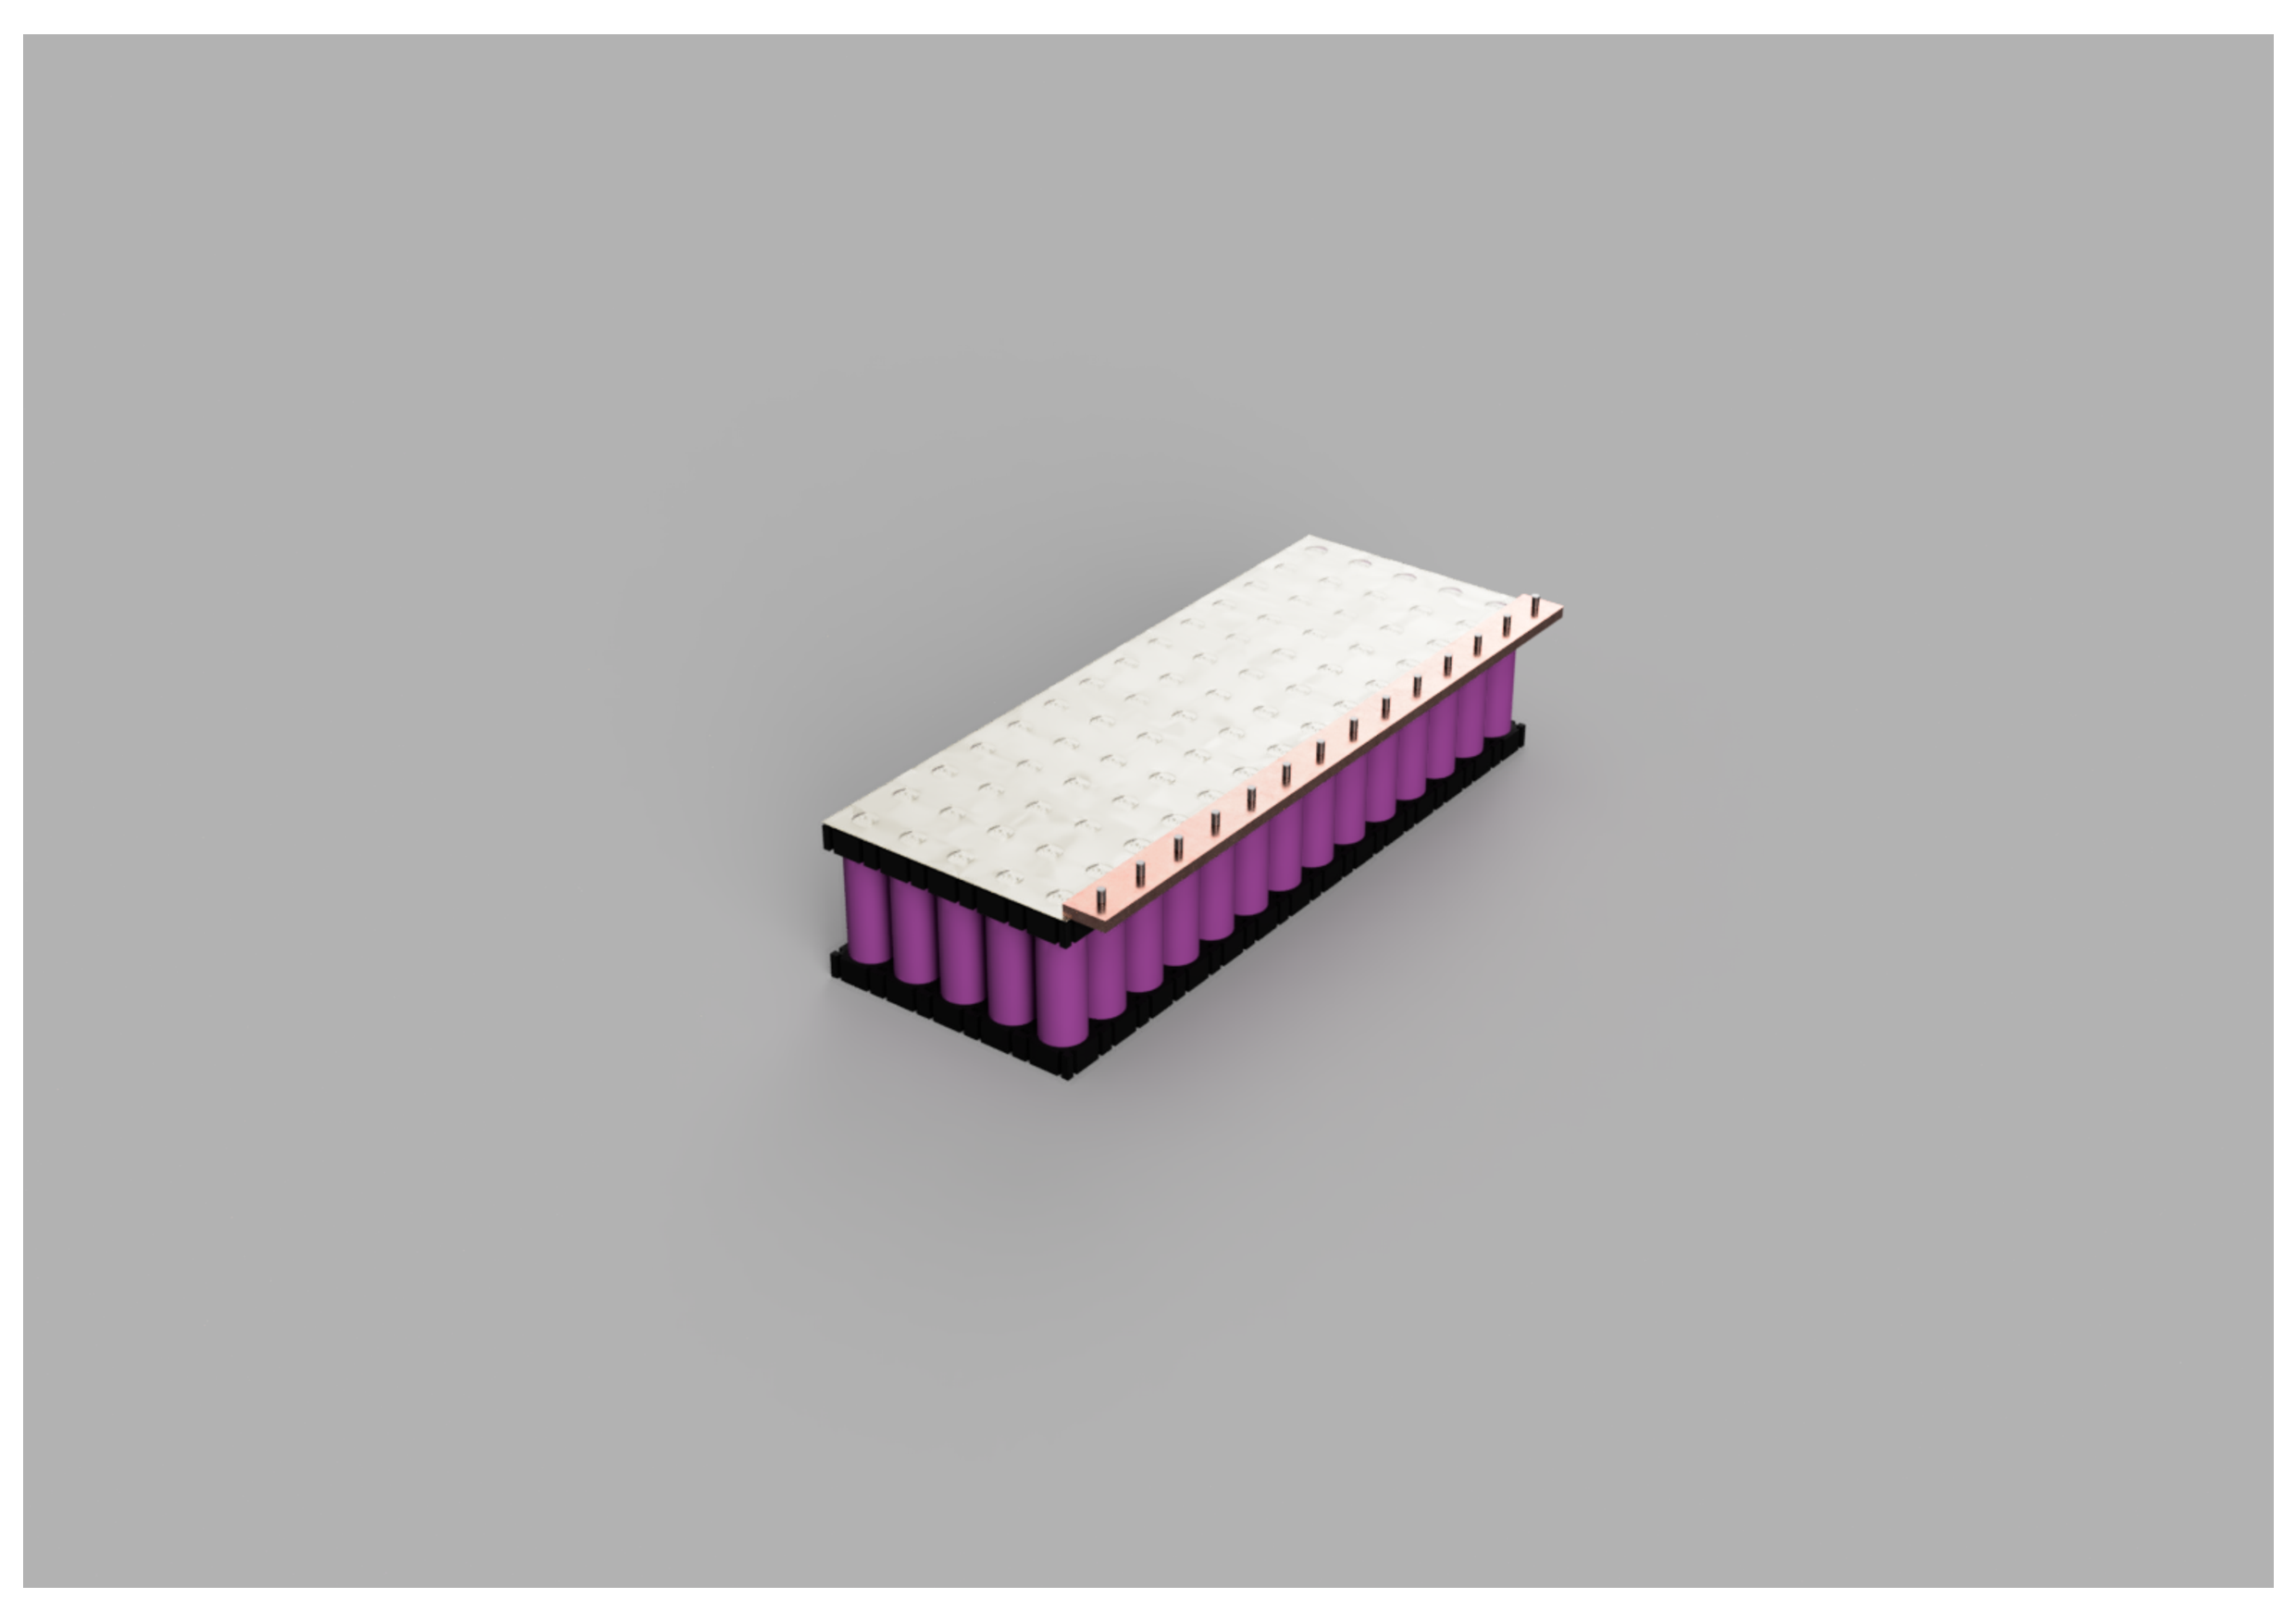
\includepdf[pages=1, fitpaper=true, pagecommand={%
	\thispagestyle{empty} % Entfernt Seitenzahlen und Kopfzeilen
	\begin{center}
		\captionof{figure}{etailed 3D CAD rendering of a lithium-ion cell used in the energy storage system.} % Fügt die Caption ein
		\label{fig:Zelle} % Für Querverweise
	\end{center}
}]{circuts/Zelle.pdf}
\addtocounter{page}{1} % Seitenzähler korrekt erhöhen

The battery pack presented in \ref{fig:Zelle}  was designed specifically for use in an electric utility vehicle—the E-Mule. In such mobile applications, energy storage must not only provide sufficient capacity and power density, but also fulfill mechanical and thermal requirements, ensure serviceability, and allow compact packaging. These constraints played a central role in the CAD modeling process and directly influenced key design decisions.

The final design was entirely created using Fusion 360, with a strong focus on modularity, manufacturability, and the physical integration of standard lithium-ion cells (type 21700). The enclosure and internal structures were tailored for additive manufacturing using PETG, a common thermoplastic with suitable strength and heat resistance \cite{gebhardt2016}. No electrical testing or thermal simulation was conducted as part of this stage; the focus remained on the mechanical layout and enclosure architecture.

\section{Detailed CAD Design Process in Fusion 360}

\subsection{Cell Holder Design and Arrangement}

The first modeling step was the design of an individual battery cell holder (\ref{fig:Zelle}). Each cell is a cylindrical 21700 lithium-ion battery, typically 21 mm in diameter and 70 mm in length. In Fusion 360, a 2D sketch was created with circular cutouts for each cell, spaced evenly in a grid pattern. These cutouts were then extruded to form vertical cavities, which securely hold the cells while leaving sufficient clearance for thermal expansion and wiring.

To ensure consistent wall thickness and clearance, the design used parameterized dimensions tied to a master sketch. This allowed rapid iteration and adjustment of the number of cells in the matrix. 

The resulting layout provides space for a total of 70 cells (14× 5 array), which was deemed sufficient for the E-Mule’s use case in terms of energy content. The precision and symmetry of the layout were maintained through pattern tools and the use of midplane construction lines.

% Assembly mit Gehäuse
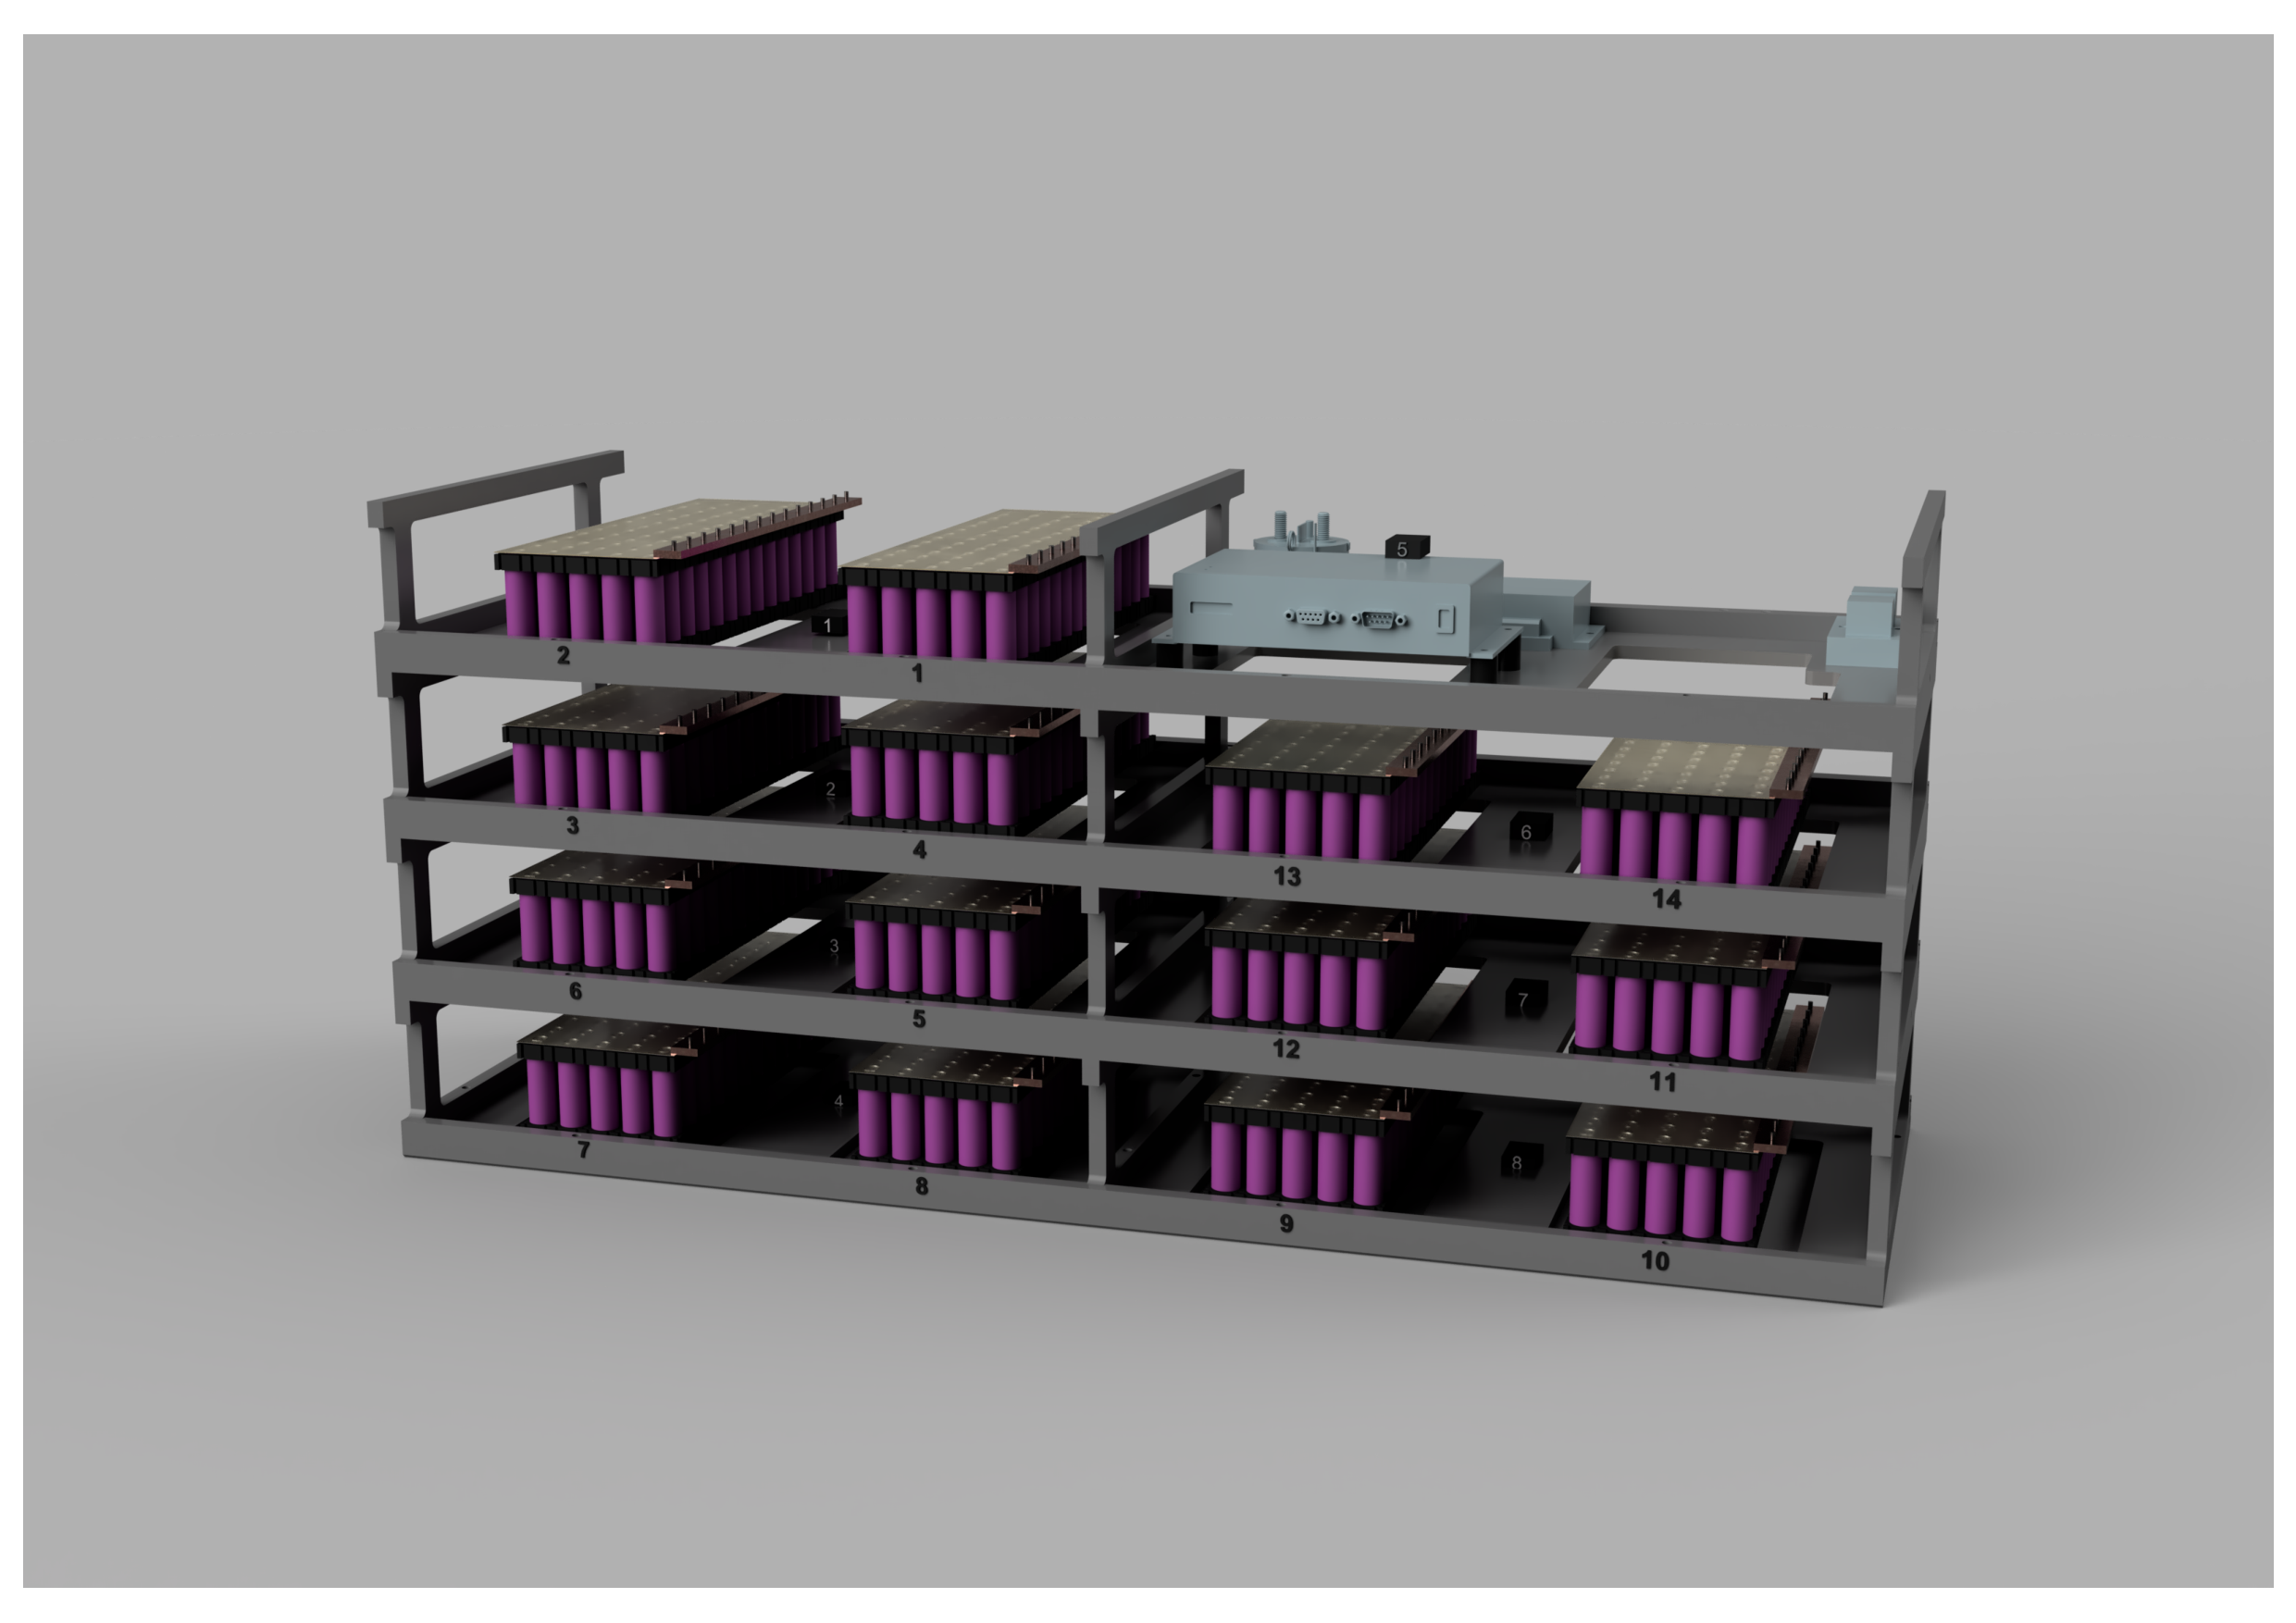
\includepdf[pages=1, fitpaper=true, pagecommand={%
	\thispagestyle{empty}
	\begin{center}
		\captionof{figure}{Fully assembled energy storage module.}
		\label{fig:Assembly}
	\end{center}
}]{circuts/Energiespeichersystem_Assembley_TOP.pdf}
\addtocounter{page}{1}

After creating the single cell holder as a component, it was duplicated and arranged in Fusion 360’s assembly environment to simulate the full module layout, seen in \ref{fig:Assembly}. This stage focused on integrating all components—holders, cell blocks, connector slots, sensor openings—into a complete mechanical structure.


During assembly, care was taken to maintain access to each row for both cooling and cabling. Clearances were checked using section analysis and interference detection tools within Fusion 360. Dummy models of power connectors and temperature sensors were placed to simulate real-world installation.



\subsection{Integration of the Protective Enclosure}
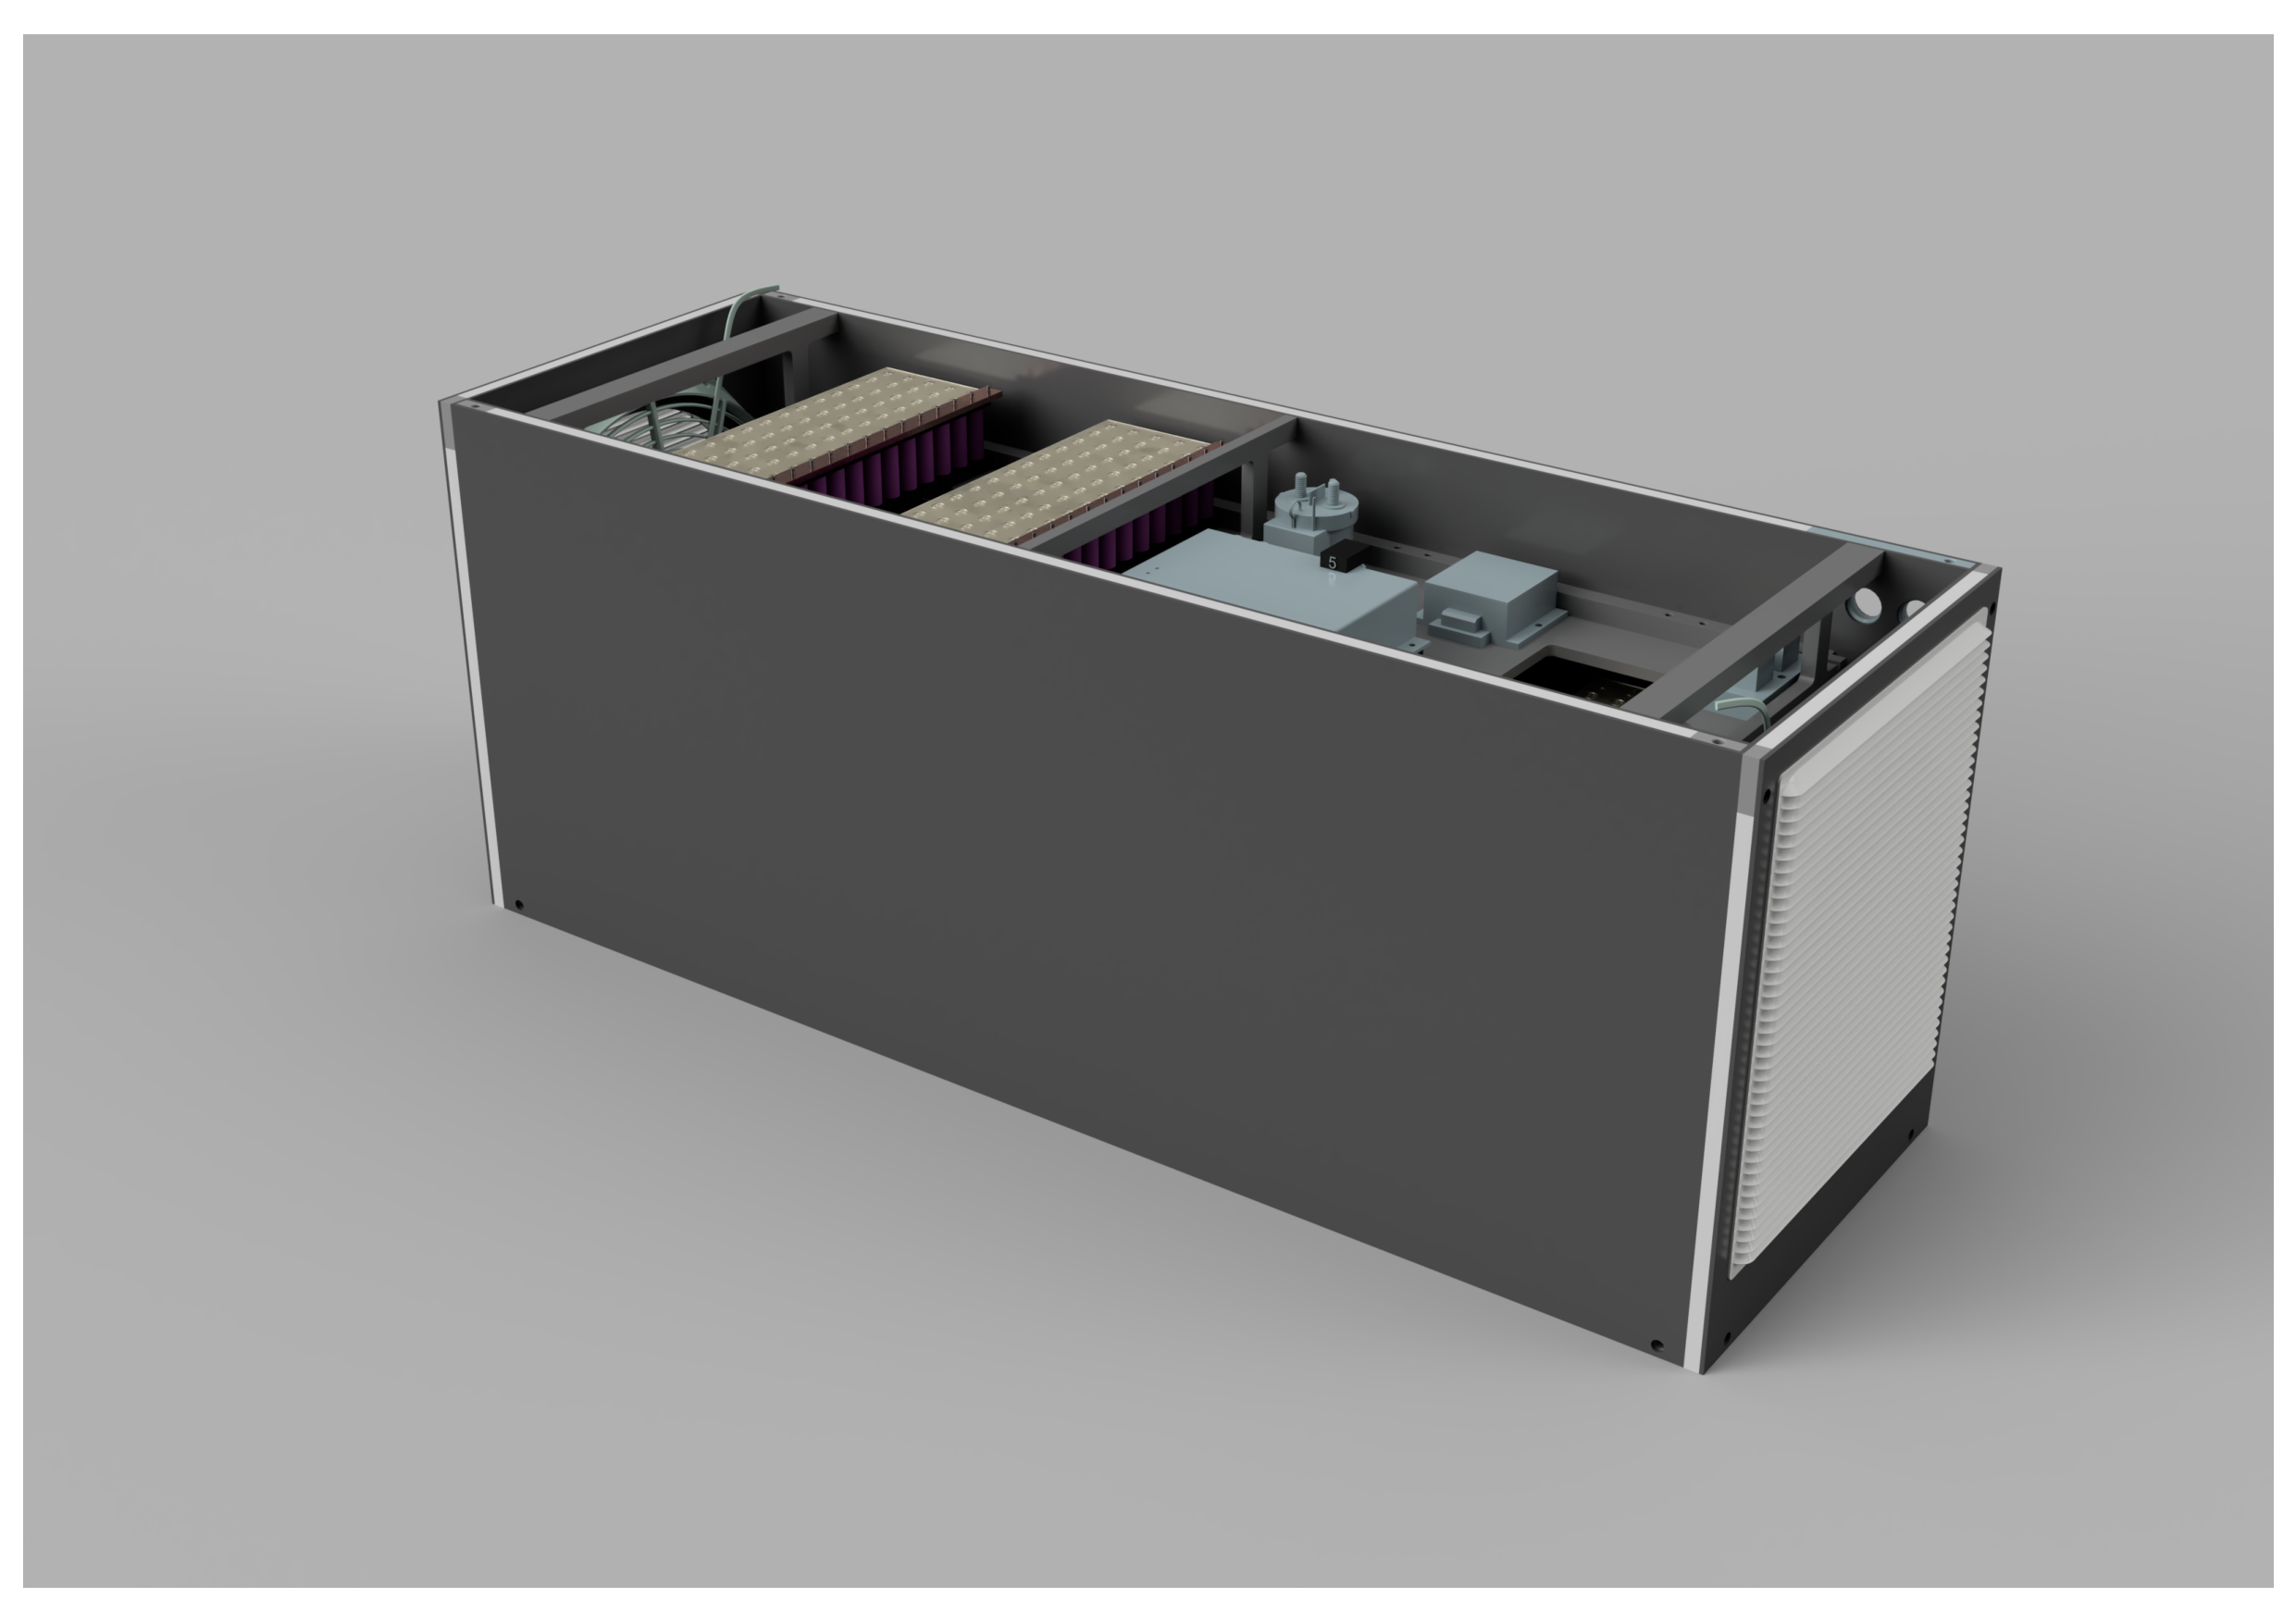
\includepdf[pages=1, fitpaper=true, pagecommand={%
	\thispagestyle{empty}
	\begin{center}
		\captionof{figure}{Fully assembled energy storage module with housing for use in the eMule vehicle.}
		\label{fig:AssemblyHousing}
	\end{center}
}]{circuts/Energiespeichersystem_Assembley_TOP_mit gehause.pdf}
\addtocounter{page}{1}
The final design step was the addition of a functional enclosure as seen in \ref{fig:AssemblyHousing}. The enclosure was modeled as a single shell body with integrated ventilation openings, flanged screw points, and access cutouts for connectors. Its purpose is to protect the cells from mechanical impact, environmental contamination, and unintentional contact.

The enclosure follows the contour of the internal components closely, minimizing unused space while allowing air to circulate between components. To accommodate additive manufacturing constraints, all overhangs were designed with a maximum angle of 45°, and fillets were added at all interior corners to prevent stress concentration. A removable lid was included to enable servicing of the battery.

The following figure illustrates the fully enclosed battery system, ready for 3D printing.

% Assembly mit Gehäuse


\section{Conclusion on the CAD Design Process}

Using Fusion 360 allowed for a highly structured, iterative, and parametric modeling workflow. All geometric relationships between components were carefully maintained, which significantly simplified later adjustments. The use of parametric sketches and pattern tools proved crucial in efficiently laying out large arrays of repetitive features, such as the cell holders.

The final result is a complete digital twin of the battery system, suited for additive manufacturing and integration in the E-Mule platform. While no physical tests or simulations were performed, the model meets the spatial, mechanical, and packaging criteria outlined at the beginning of the project.


\chapter{Zusammenfassung}
\label{cha:zusammenfassung}

%Auf zwei bis drei Seiten soll auf folgende Punkte eingegangen werden:


	%\item Welches Ziel sollte erreicht werden
	Im Rahmen des Projekts eMule 7.0 wurden verschiedene Ziele für das Wintersemester 2024 gesetzt. Diese lauteten:
	\begin{itemize}
		\item[1.] Fortsetzung der Entwicklung und Installation des neuen Energiespeichersystems in Form einer Traktionsbatterie für das eMule-Fahrzeug
		\item[2.] Weiterentwicklung des Kühlsystems der Traktionsbatterie
		\item[3.] Verbesserung der vorhandenen Kühlsystem-Temperaturregelung durch Arduino-Mikrocontrollerprogrammierung
		\item[4.] Verbesserung der Verkabelung des vorhandenen Tranktionsbatteriemanagementsystems
		\item[5.] Einbau von Sensoren
		\item[6.] Erstellung von aktuellen Stromlauf und Bestückungsplänen der elektrisch/elektronischen Fahrzeugschaltkreise
		\item[7.] Vereinheitlichung und Vergemeinschaftung der Pläne des Systems und dessen Einzelkomponenten
		\item[8.] Erstellung einer Installationsanleitung für Autodesk Fusion 360 für verschiedene Betriebssysteme
		\item[9.]Durchführung von Messungen und Funktionstests
		\item[10.] Vorbereitung des Fahrzeugs für die bevorstehende EMV-Prüfung und TÜV-Abnahme
	\end{itemize}
Da in dieser Arbeit lediglich die Ziele sechs bis acht betrachtet wurden wird auch nur auf diese weiter eingegangen. \newline
Um die Erstellung aktueller Stromlaufpläne möglichst effizient zu gestalten wurden zwei verschiedene Vorgehen angewendet. Mussten bereits vorhandene Pläne lediglich aktualisiert werden wurde wie folgt vorgegangen:\newline
Für die Aktualisierung der Stromlauftpläne nach festgelgter Norm und aktuellem Verbaustand wurden der vorliegende Plan zunächst ausgedruckt. Im ersten Schritt wurden diese Stromlaufpläne systematisch auf Unstimmigkeiten, wie fehlende Verbindungen oder unklare Symbolik, überprüft. Gefundene Fehler wurden im nächsten Schritt markiert und anschließend korrigiert, wodurch die Einhaltung elektrotechnischer Standards gewährleistet werden konnte. Zudem erfolgte eine Layoutanpassung zur Verbesserung der Übersichtlichkeit. Im letzten Schritt wurde herausgefunden, nach welcher Norm der Stromlaufplan erstellt wurde. Diese Norm wurde recherchiert und in die von uns gewählte DIN EN 60617 Norm \glqq übersetzt\grqq {}. Die überarbeiteten Stromlaufpläne wurden abschließend mit Autodesk Fusion 360 in ein DIN-A3-Format übertragen. Durch die Integration von Titelblock und Legende konnte die Professionalität und Lesbarkeit sichergestellet werden. \newline
Es wurden Stromlaufpläne für sämtliche Systemteile, die zum Zeitpunkt der veröffentlichug dieser Arbeit finalisiert waren, erstellt. Diese Stromlaufpläne entsprechen den Standarts der DIN EN 60617, sind in einheitlicher Form erstellt und in einem übergeordneten Gesamtprojekt vergemeinschaftet. Insgesamt wurden somit fünf Stromlaufpläne realisiert. Aufgrund interner Absprachen wurde die Erstellung der Bestückungspläne in den nächsten Bearbeitungszeitraum im Sommersemester 2025 verschoben. Im Rahmen der Pläneerstellung wurde das Team sehr gut in das Programm Autodesk Fusion 360 eingearbeitet, eine eigene Bibliothek zur DIN EN 60617 angelegt und eine Struktur zur einfachen Erweiterung der Vergemeinschaftung aufgebaut. Weiter konnte sichergestellt werden, dass neue Teammitglieder einfach zu der Projektcloud hinzugefügt werden können, sowie eine detailierte Anleitung zur Installation der CAD-Softwäre auf sämtlichen Betriebssystemen zur Verfügung gestellt bekommen haben. Zusätzlich wurde der Installtionsvorgang der Software auf den laborinternen Geräten gestartet. Neben den Teamspezifischen Aufgaben konnten die anderen Projektteams bei diversen Aufgaben unterstützt werden. Hierzu zählen beispielsweise das Verladen und damit verbundenen Ein- und Ausbau der Batterie in das Fahrzeug oder die Bohrung zusätzlicher Löcher in die Aussenwand der Tragfläche des Fahrzeugs um eine bessere Funktionalität der Lüfter sicherzustellen.


%In der Zusammenfassung sind unbedingt klare Aussagen zum Ergebnis der Arbeit zu nennen. Üblicherweise können Ergebnisse nicht nur qualitativ, sondern auch quantitativ benannt werden, z.~B. \glqq \ldots konnte eine Effizienzsteigerung von \SI{12}{\percent} erreicht werden.\grqq~oder \glqq \ldots konnte die Prüfdauer um \SI{2}{\hour} verkürzt werden\grqq.

%Die Ergebnisse in der Zusammenfassung sollten selbstverständlich einen Bezug zu den in der Einleitung aufgeführten Fragestellungen und Zielen haben.
\section{Ausblick}
Zwischen dem gerade vergangenen Arbeitszeitraum \glqq Wintersemester 2024 \grqq und dem kommenden Arbeitszeitraum \glqq Sommersemester 2025 \grqq werden alle Team, in reduziertem Rahmen nach Bedarf und Möglichkeit,  ihre Aufgaben fortführen. Weiter ist eine TÜV-Abnahme für das Fahrzeug geplant.\newline
Im nächsten Arbeitszeitraum sollen dann ergänzend zu der nach aktuellem Stand vorhanden Dokumentation weitere Stromlaufpläne generiert und in diese aufgenommen werden. Neben Stromlaufplänen soll die Dokumentation durch Bestückungspläne erweitert werden. Um die Übersichtlichkeit weiter zu verbessern soll die gesamte Dokumentation in einem großen Dokument als Gesamtprojekt mit sämtlichen Projekttiefen festgehalten werden. Weitere Ziele für das nächste Semester umfassen eine Modularisierung der Batterie, den Einbau des Bussystems an die Batterie, eine Erweiterung der Temeraturüberwachung sowie die Modularisierung der Powerbox und die Installation eines Displays im Cockpit, welches sämtliche Fahr-, Verbrauchs-, und Leistungsdaten anzeigt. Als optionales Ziel soll bei entsprechendem Fortschritt des Systems noch eine Musikanlage verbaut werden.


% ---- Literaturverzeichnis ----------
\interlinepenalty 10000					% Verhindert einen Umbruch mitten in Literatureinträgen
\printbibliography						% Erstellen des Literaturverzeichnisses
\interlinepenalty 0
\clearpage

% -----Ausgabe aller Verzeichnisse ---
\setlength{\parskip}{0.5\baselineskip}

% Alle Abkürzungen, die in der Arbeit verwendet werden. Die Alphabetische Sortierung übernimmt Latex. Nachfolgend sind Beispiele genannt, welche nach Bedarf angepasst, gelöscht oder ergänzt werden können.
% Die Angaben in der eckigen Klammer werden zur Sortierung der Einträge verwendet. Vor allem bei Formelzeichen hat man sonst das Problem, dass diese möglicherweise nicht wie gewünscht sortiert werden.

% Bei den unten stehenden Formelzeichen ist erläutert, wie explizite Sortierschlüssel über den Inhalt der eckigen Klammer angegeben werden.

% Zum Aktualisieren des Abkürzungsverzeichnisses (Nomenklatur) bitte auf der Kommandozeile folgenden Befehl aufrufen :
% makeindex <Dateiname>.nlo -s nomencl.ist -o <Dateiname>.nls
% Oder besser: Kann in TexStudio unter Tools-Benutzer als Shortlink angelegt werden
% Konfiguration unter: Optionen-Erzeugen-Benutzerbefehle: makeindex -s nomencl.ist -t %.nlg -o %.nls %.nlo

% Allgemeine Abkürzungen %%%%%%%%%%%%%%%%%%%%%%%%%%%%
%\nomenclature[Abb]{Abb.}{Abbildung}
%\nomenclature[bzw]{bzw.}{beziehungsweise}
%\nomenclature[DHBW]{DHBW}{Duale Hochschule Baden-Württemberg}
%\nomenclature[ebd]{ebd.}{ebenda}
%\nomenclaturev[etal]{et al.}{at alii}
%\nomenclature[etc]{etc.}{et cetera}
%\nomenclature[evtl]{evtl.}{eventuell}
\nomenclature[f]{f.}{folgende Seite}
%\nomenclature[ff]{ff.}{fortfolgende Seiten}
%\nomenclature[ggf]{ggf.}{gegebenenfalls}
%\nomenclature[Hrsg]{Hrsg.}{Herausgeber}
%\nomenclature[Tab]{Tab.}{Tabelle}
%\nomenclature[ua]{u. a.}{unter anderem}
%\nomenclature[usw]{usw.}{und so weiter}
\nomenclature[vgl]{vgl.}{vergleiche}
\nomenclature[zB]{z. B.}{zum Beispiel}
\nomenclature[HV]{HV}{High Voltage}
\nomenclature[LV]{LV}{Low Voltage}
\nomenclature[CC]{CC}{Constant Current}
\nomenclature[CV]{CV}{Constant Voltage}
\nomenclature[DIN]{DIN}{Deutsche Industrie Norm}
\nomenclature[IEC]{IEC}{Inernational Electrotechnical Commission}
\nomenclature[ANSI]{ANSI}{American National Standards Institute}
\nomenclature[CAD]{CAD}{Computer-Aided Design}
\nomenclature[EMV]{EMV}{Elektromagnetische Verträglichkeit}
\nomenclature[TÜV]{TÜV}{Technischer Überwachungsverein}
\nomenclature[CAM]{CAM}{Computer-Aided Manufacturing}
\nomenclature[CAE]{CAE}{Computer-Aided Engineering}
\nomenclature[Inc]{Inc}{Incorporated}
\nomenclature[EN]{EN}{Europäische Norm}
\nomenclature[PTC]{PTC}{Positive Temperature Coefficient}
\nomenclature[LED]{LED}{Light Emitting Diode}
%\nomenclaturev[zT]{z. T.}{zum Teil}

% Dateiendungen %%%%%%%%%%%%%%%%%%%%%%%%%%%%%%%%%%%%
%\nomenclature[EMF]{EMF}{Enhanced Metafile}
%\nomenclature[JPG]{JPG}{Joint Photographic Experts Group}
\nomenclature[KI]{KI}{Künstliche Intelligenz}
\nomenclature[PDF]{PDF}{Portable Document Format}
\nomenclature[PNG]{PNG}{Portable Network Graphics}
%\nomenclature[]{XML}{Extensible Markup Language}

% Abkürzungen von Fachbegriffen %%%%%%%%%%%%%%%%%%%%
%\nomenclature[ABS]{ABS}{Antiblockiersystem}
%\nomenclature[ESC]{ESC}{Electronic Stability Control, Fahrdynamikregelung}

% Formelzeichen %%%%%%%%%%%%%%%%%%%%%%%%%%%%%%%%%%%%
%\nomenclature[a]{$a$}{Beschleunigung}
%%%%%\nomenclature[R]{$R$}{Widerstand}


				% Datei mit allgemeinen Abkürzungen laden
\renewcommand{\nomname}{Verzeichnis verwendeter Formelzeichen und Abkürzungen}
%\addcontentsline{toc}{chapter}{\nomname}
\setlength{\nomlabelwidth}{.20\hsize}
\renewcommand{\nomlabel}[1]{#1 \dotfill}
\setlength{\nomitemsep}{-\parsep}
\printnomenclature						% Erzeugen des Abkürzungsverzeichnises, siehe auch Inhalt der Datei pages/abkuerzungen.tex
\clearpage

\listoffigures 							% Erzeugen des Abbildungsverzeichnisses 
\clearpage

\listoftables 							% Erzeugen des Tabellenverzeichnisses
\clearpage

% -----Anhang ------------------------

\appendix
%\pagenumbering{Roman}					% große, römische Seitenzahlen für Anhang, falls gewünscht
\addchap{Use of artificial intelligence-based tools}
\setcounter{chapter}{1}

%Im Rahmen dieser Arbeit wurden Künstliche Intelligenz (KI)\index{Künstliche Intelligenz} basierte Werkzeuge benutzt. Tabelle~\ref{tab:anhang_uebersicht_KI_werkzeuge} gibt eine Übersicht über die verwendeten Werkzeuge und den jeweiligen Einsatzzweck.
Artificial intelligence (AI)\index{Artificial intelligence} based tools were used in this work. Table~\ref{tab:anhang_uebersicht_KI_werkzeuge} provides an overview of the tools used and their respective purpose.

\begin{table}[hbt]	
	\centering
	\renewcommand{\arraystretch}{1.5}	% Skaliert die Zeilenhöhe der Tabelle
	\captionabove[Liste der verwendeten Künstliche Intelligenz basierten Werkzeuge]{Liste der verwendeten KI basierten Werkzeuge}
	\label{tab:anhang_uebersicht_KI_werkzeuge}
	\begin{tabular}{>{\raggedright\arraybackslash}p{0.3\linewidth} >{\raggedright\arraybackslash}p{0.65\linewidth}}
		\textbf{Werkzeug} & \textbf{Beschreibung der Nutzung}\\
		\hline 
		\hline
		Mercedes-Benz Direct Chat & 	\vspace{-\topsep}
					\begin{itemize}[noitemsep,topsep=0pt,partopsep=0pt,parsep=0pt] 
						\item Formulierungshilfe und Rechtschreibprüfung (siehe gesamte Arbeit)
				   	\end{itemize} \\
		DeepL	&	\vspace{-\topsep}
					\begin{itemize}[noitemsep,topsep=0pt,partopsep=0pt,parsep=0pt] 
					\item Übersetzung der Arbeit 
					\end{itemize} \\ 
	\end{tabular} 
\end{table}

%\addchap{B Ergänzungen}
%\setcounter{chapter}{2}

%\section{Details zu bestimmten theoretischen Grundlagen}

%\section{Weitere Details, welche im Hauptteil den Lesefluss behindern}

%\addchap{C Details zu Laboraufbauten und Messergebnissen}
%\setcounter{chapter}{3}
%\setcounter{section}{0}
%\setcounter{table}{0}
%\setcounter{figure}{0}

%\section{Versuchsanordnung}

%\section{Liste der verwendeten Messgeräte}

%\section{Übersicht der Messergebnisse}

%\section{Schaltplan und Bild der Prototypenplatine}

%\addchap{D Zusatzinformationen zu verwendeter Software}
%\setcounter{chapter}{4}
%\setcounter{section}{0}
%\setcounter{table}{0}
%\setcounter{figure}{0}

%\section{Struktogramm des Programmentwurfs}

%\section{Wichtige Teile des Quellcodes}

%\addchap{E Datenblätter}
%\setcounter{chapter}{5}
%\setcounter{section}{0}
%\setcounter{table}{0}
%\setcounter{figure}{0}

%\section{Einbinden von PDF-Seiten aus anderen Dokumenten}

%Auf den folgenden Seiten wird eine Möglichkeit gezeigt, wie aus einem anderen PDF-Dokument komplette Seiten übernommen werden können, z.~B. zum Einbindungen von Datenblättern. Der Nachteil dieser Methode besteht darin, dass sämtliche Formateinstellungen (Kopfzeilen, Seitenzahlen, Ränder, etc.) auf diesen Seiten nicht angezeigt werden. Die Methode wird deshalb eher selten gewählt. Immerhin sorgt das Package \textit{\glqq pdfpages\grqq}~für eine korrekte Seitenzahleinstellung auf den im Anschluss folgenden \glqq nativen\grqq~\LaTeX-Seiten.

%Eine bessere Alternative ist, einzelne Seiten mit \textit{\glqq$\backslash$includegraphics\grqq}~einzubinden.

%
\includepdf[pages={2-4}]{docs/EingebundenesPDF.pdf}

%\clearpage

\clearpage

%\addchap{F Tips und Beispiele zu \LaTeX-Befehlen}
\setcounter{chapter}{6}
\setcounter{section}{0}
\setcounter{table}{0}
\setcounter{figure}{0}

Dieses Kapitel können Sie einfach löschen, indem Sie in der Präambel am Anfang der Zeile \glqq \textbackslash\textit{include\{chapter/anhang\lowrule vorlagen\}}\grqq~das Symbol \% zum Auskommentieren einfügen.

\section{Wichtige \LaTeX -Befehle}

\begin{tabbing}
\hspace*{0cm} \= \hspace{0.42\linewidth} \= \+\kill
\textbackslash \textit{label}\{\}	\> Definition eines Labels, auf welches referenziert \\ 
	\> werden kann, z.~B.: \textbackslash \textit{label}\{fig:MyImage\}\\ 
\textbackslash \textit{ref}\{\}	\> Setzen einer Referenz zu einem Label\\
\> z.~B.: \ldots siehe Tabelle\~{}\textbackslash \textit{ref}\{tab:messdaten\}.\\ 
\textbackslash \textit{pageref}\{\}	\> Gibt die Seitenzahl zu einer Referenz zurück\\

	\textbackslash \textit{autocite}\{\}	\> Literaturreferenz einfügen\\
	\textbackslash \textit{autocite}[7]\{\}	\> Literaturreferenz einfügen, hier mit zus. Referenz\\
	\> auf Seite 7\\
\textbackslash \textit{autocites}\{Abc15, Def16\}	\> Mehrere Literaturreferenzen, hier Abc15 und \\
\> Def16, einfügen\\
\textbackslash \textit{footnote}\{\}	\> Fußnote einfügen\\ 
\~{}	\> Einfügen eines geschützten Leerzeichens\\ 
\textdollar \textit{Formel} \textdollar	\> Eingabe einer Formel im Text\\
\textdollar\textit{l}=\textbackslash \textit{SI}\{10\}\{\textbackslash \textit{meter}\}\textdollar	\> Korrekte Ausgabe Maßzahl und Einheit in\\
\> Formeln, hier $l=\SI{10}{\meter}$\\
\textbackslash \textit{index}\{Kraft\} \> Aufnahme des Begriffs \glqq Kraft\grqq~in das Sachwort- \index{Kraft} \\
\> verzeichnis\\
\textbackslash \textit{index}\{Induktion!Vollständige\} \> Aufnahme des Begriffs \glqq Vollständige\grqq~in das Sach-\\
\> wortverzeichnis unter \glqq Induktion\grqq. \index{Induktion!Vollständige} \\
\textbackslash \textit{nomenclature}[etc]\{etc.\}\{et cetera\}	\> Aufnahme der Abkürzung \glqq etc.\grqq~für \glqq et cetera\grqq~in \\
\> das Abkürzungsverzeichnis. Die Angabe [etc] dient\\
\>als Sortierschlüssel\\
\textbackslash \textit{clearpage}	\> Ausgabe aller Gleitobjekte und Umbruch auf eine\\
\> neue Seite\\ 
\end{tabbing}

\clearpage

\section{Vorlagen für \LaTeX Umgebungen}

\subsection{Listen und Aufzählungen}

Es gibt folgende Listentypen. Die wichtigsten:

\begin{itemize}
	\item Einfache Liste mit \textit{itemize}-Umgebung
	\item ...
\end{itemize}

\begin{enumerate}
	\item Nummerierte Liste mit \textit{enumerate}-Umgebung
	\item ...
\end{enumerate}

\begin{enumerate}[label=\alph*.]
	\item wobei man bei der \textit{enumerate}-Umgebung leicht die Art der Nummerierung ändern kann,
	\item ...
\end{enumerate}

und durch verschachtelte Umgebungen verschiedene Aufzählungsebenen darstellen kann:

\begin{enumerate}[label=\alph*)]
	\item Erster Aufzählungspunkt der ersten Ebene
	\item ...
	\begin{itemize}
		\item Erster Punkt der zweiten Ebene
		\item Zweiter Punkt der zweiten Ebene
	\end{itemize}
	\item Das sollte an Beispielen zunächst einmal genügen.
\end{enumerate}

\clearpage

\subsection{Bilder und Grafiken}

Bilder können als PDF-, JPG-, und PNG-Bilder in \LaTeX eingebunden werden. Damit eine Grafik in hoher Qualität dargestellt wird, sollte das Dateiformat der Grafik vektorbasiert sein, d.h. als PDF-Datei vorliegen. Viele Zeichenprogramme unterstützen einen PDF-Export (z.~B. GIMP, Adobe Illustrator, etc.). Für Grafiken aus PowerPoint sei folgende Vorgehensweise beim Export empfohlen:

\begin{enumerate}
	\item Die gewünschte Grafik in PowerPoint zeichnen.
	\item Gewünschten Bildbereich markieren, rechte Maustaste klicken und \glqq Als Grafik speichern ...\grqq~wählen.
	\item Grafik im Format EMF abspeichern. Das EMF-Format ist vektorbasiert.\footnote{Mit dem Mac kann in PowerPoint die Grafik direkt im PDF-Format exportiert werden. Die weiteren Schritte entfallen daher.}
	\item Mit dem Programm XnView die Grafik im EMF-Format in PDF wandeln und abspeichern.
	\item Die so erzeugte PDF-Datei enthält eine vektorbasierte Grafik und kann in \LaTeX~ eingebunden werden.
\end{enumerate}

Abbildung~\ref{fig:MyImage} zeigt ein Beispielbild einer Grafik, welche aus PowerPoint exportiert wurde.

\begin{figure}[hbt]
	\centering
	
\includegraphics[width=0.3\linewidth]{images/MyImage}
	\caption[Beispiel für die Einbindung eines Bildes.]{Beispiel für die Einbindung eines Bildes (PDF-, JPG-, und PNG-Bilder können eingebunden werden).}
	\label{fig:MyImage}
\end{figure}

Der Quellcode des Beispielbildes aus Abbildung~\ref{fig:MyImage} ist in Listing~\ref{lst:fig} zu sehen.

\clearpage

\begin{lstlisting}[caption=Quellcode der Abbildung~\ref{fig:MyImage}.,label=lst:fig]
\begin{figure}[hbt]				% here, bottom, top
\centering						% Zentrierung

\includegraphics[width=0.6\linewidth]{images/MyImage}		
\caption[Beispiel für die Einbindung eines Bildes.]{Beispiel für die Einbindung eines Bildes (PDF-, JPG-, und PNG-Bilder können eingebunden werden).}
\label{fig:MyImage}
\end{figure}
\end{lstlisting}

Jedes Bild aus fremder Quelle ist mit einem Zitat in der Abbildungsunterschrift zu kennzeichnen. Nur eigene Bilder benötigen keine entsprechende Kennzeichnung. Bilder aus fremder Quelle mit eigenen Ergänzungen oder Änderungen sind mit Zitat und einer entsprechenden Bemerkung (z. B. \glqq auf Basis [Quelle] mit eigenen Ergänzungen\grqq~oder \glqq eigene Darstellung auf Basis [Quelle]\grqq) zu versehen. Der besseren Lesbarkeit halber sind im Abbildungsverzeichnis keine Zitate anzugeben. Hierfür kann im Befehl \textbackslash \textit{caption[]\{\}} innerhalb der eckigen Klammer eine modifizierte Abbildungsunterschrift eingegeben werden, welche in das Abbildungsverzeichnis übernommen wird. Der Text innerhalb der geschweiften Klammer wird direkt unter die Abbildung gedruckt und kann dagegen ausführlich mit Angabe eines Zitats sein. Sollte die Arbeit veröffentlicht werden, ist unbedingt darauf zu achten, dass nur dann Bilder von fremder Quelle übernommen werden dürfen, wenn hierfür das explizite Einverständnis des Urhebers vorliegt. Dieses Einverständnis ist persönlich einzuholen und separat zu dokumentieren.

Grafiken können auch mithilfe des Packages Tikz gezeichnet, bzw. programmiert werden. Grafiken mit Tikz werden mit dem \textit{input}-Befehl in die \textit{figure}-Umgebung geladen, wie nachfolgendes Beispiel in Abbildung~\ref{fig:tikz_house} zeigt:

\begin{figure}[hbt]
	\centering
	 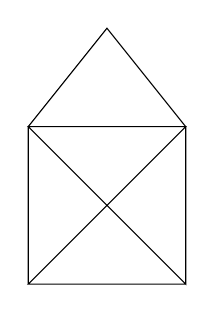
\begin{tikzpicture}
\draw (0,0) -- (0,2) -- (1,3.25) -- (2,2) -- (2,0) -- (0,2) -- (2,2) -- (0,0) -- (2,0);
\end{tikzpicture}
    
	\caption[Mit Tikz programmierte Grafik.]{Mit Tikz programmierte Grafik.}
	\label{fig:tikz_house}
\end{figure}

Ein etwas umfangreicheres Beispiel zur Digitaltechnik ist in Abbildung~\ref{fig:tikz_digital} dargestellt:

\begin{figure}[hbt]
	\centering
	\usetikzlibrary{circuits.logic.US,circuits.logic.IEC}
      \begin{tikzpicture}[circuit logic US]
      \matrix[column sep=7mm]
      {
      \node (i0) {0}; & & \\
      & \node [and gate] (a1) {}; & \\
      \node (i1) {0}; & & \node [or gate] (o) {};\\
      & \node [nand gate] (a2) {}; & \\
      \node (i2) {1}; & & \\
      };
      \draw (i0.east) -- ++(right:3mm) |- (a1.input 1);
      \draw (i1.east) -- ++(right:3mm) |- (a1.input 2);
      \draw (i1.east) -- ++(right:3mm) |- (a2.input 1);
      \draw (i2.east) -- ++(right:3mm) |- (a2.input 2);
      \draw (a1.output) -- ++(right:3mm) |- (o.input 1);
      \draw (a2.output) -- ++(right:3mm) |- (o.input 2);
      \draw (o.output) -- ++(right:3mm) node [right] {$y$ \quad Hier könnte Ihre Formel $y=(0 \land 0) \lor \overline{( 0 \land 1)}$ stehen};
 \end{tikzpicture}

	\caption[Mit Tikz programmierte Grafik, welche bereits vorgefertigte Bibliotheken für Symbole aus der Digitaltechnik nutzt.]{Mit Tikz programmierte Grafik, welche bereits vorgefertigte Bibliotheken für Symbole aus der Digitaltechnik nutzt.}
	\label{fig:tikz_digital}
\end{figure}

%\clearpage

In der Tikz-Umgebung können auch Diagramme mit dem \textit{pgfplot}-Befehlssatz erzeugt werden. In Abbildung \ref{fig:pgfplot} sehen Sie ein Beispiel.

\begin{figure}[hbt]
	\centering
	\begin{tikzpicture}
		\begin{axis}[scale=1.3,legend entries={Messwerte mit Fehlerbalken,
			$\pgfmathprintnumber{\pgfplotstableregressiona} \cdot x  
			\pgfmathprintnumber[print sign]{\pgfplotstableregressionb}$}, legend style={draw=none},legend style={at={(0.01,0.98)},anchor=north west},xlabel=Stromstärke $I \; \mathrm{ \lbrack mA \rbrack}$,ylabel=Spannung $U \; \mathrm{ \lbrack V \rbrack}$]
		\addlegendimage{mark=*,blue}
		\addlegendimage{no markers,red}
\addplot+[error bars/.cd, y dir=both,y explicit]
table[x=x,y=y,y error=errory] 
{pgfplot/messdaten_mitfehler.dat};
\addplot table[mark=none,y={create col/linear regression={y=y}}]
{pgfplot/messdaten_mitfehler.dat};
	\end{axis}
\end{tikzpicture}
	\caption[Diagramm, erstellt mit dem \textit{pgfplot}-Befehlssatz.]{Ein Diagramm, erstellt in der \textit{tikzpicture}-Umgebung mit dem \textit{pgfplot}-Befehlssatz. Das Diagramm stellt Messdaten, deren Fehlerbalken und eine Regressionskurve dar. Die Messdaten werden von einer separaten Datei eingelesen und die Regressionskurve wurde mit \textit{pgfplot} berechnet und erstellt.}
	\label{fig:pgfplot}
\end{figure}

\clearpage

Auch hierzu der Quellcode in Listing~\ref{lst:pgfplot}.

\begin{lstlisting}[caption=Quellcode der Abbildung~\ref{fig:pgfplot}.,label=lst:pgfplot]
\begin{figure}[hbt]
\centering
\begin{tikzpicture}
		\begin{axis}[scale=1.3,legend entries={Messwerte mit Fehlerbalken,
			$\pgfmathprintnumber{\pgfplotstableregressiona} \cdot x  
			\pgfmathprintnumber[print sign]{\pgfplotstableregressionb}$}, legend style={draw=none},legend style={at={(0.01,0.98)},anchor=north west},xlabel=Stromstärke $I \; \mathrm{ \lbrack mA \rbrack}$,ylabel=Spannung $U \; \mathrm{ \lbrack V \rbrack}$]
		\addlegendimage{mark=*,blue}
		\addlegendimage{no markers,red}
\addplot+[error bars/.cd, y dir=both,y explicit]
table[x=x,y=y,y error=errory] 
{pgfplot/messdaten_mitfehler.dat};
\addplot table[mark=none,y={create col/linear regression={y=y}}]
{pgfplot/messdaten_mitfehler.dat};
	\end{axis}
\end{tikzpicture}
\caption[Diagramm, erstellt mit dem \textit{pgfplot}-Befehlssatz.]{Ein Diagramm, erstellt in der \textit{tikzpicture}-Umgebung mit dem \textit{pgfplot}-Befehlssatz. Das Diagramm stellt Messdaten, deren Fehlerbalken und eine Regressionskurve dar. Die Messdaten werden von einer separaten Datei eingelesen und die Regressionskurve wurde mit \textit{pgfplot} berechnet und erstellt.}
\label{fig:pgfplot}
\end{figure}
\end{lstlisting}

In Listing~\ref{lst:tikz} ist der Quellcode der Datei \textit{mess\_fehlerbalken.tex} dargestellt.

\begin{lstlisting}[caption=Quellcode der Datei \textit{mess\_fehlerbalken.tex}.,label=lst:tikz]
\begin{tikzpicture}
\begin{axis}[scale=1.3,legend entries={Messwerte mit Fehlerbalken,
$\pgfmathprintnumber{\pgfplotstableregressiona} \cdot x  
\pgfmathprintnumber[print sign]{\pgfplotstableregressionb}$}, legend style={draw=none},legend style={at={(0.01,0.98)},anchor=north west},xlabel=Stromstärke $I \; \mathrm{ \lbrack mA \rbrack}$,ylabel=Spannung $U \; \mathrm{ \lbrack V \rbrack}$]
\addlegendimage{mark=*,blue}
\addlegendimage{no markers,red}
\addplot+[error bars/.cd, y dir=both,y explicit]
table[x=x,y=y,y error=errory] 
{pgfplot/messdaten_mitfehler.dat};
\addplot table[mark=none,y={create col/linear regression={y=y}}]
{pgfplot/messdaten_mitfehler.dat};
\end{axis}
\end{tikzpicture}
\end{lstlisting}

\clearpage

In Abbildung~\ref{fig:pgfplot2y} wird ein weiters Beispiel für ein Diagramm gezeigt. Oftmals wird eine zweite y-Achse verwendet, um verschiedene Skalen darstellen zu können.

\begin{figure}[hbt]
	\centering
	\begin{tikzpicture}
%
\begin{axis}[
scale=1.3,
ytick pos=left,
xlabel=Zeit $t \; \mathrm{ \lbrack ns \rbrack}$,
ylabel=Spannung $U \; \mathrm{ \lbrack V \rbrack}$
]
\addplot[mark=*,only marks] table[x=x,y=y1] {pgfplot/messdaten_zweiyachsen.dat};
\end{axis}
%
\begin{axis}[
scale = 1.3,
legend style={draw=none},
legend style={at={(0.75,0.6)},
anchor=north west},
axis y line*=right,
axis x line=none,
%ymin=0,
%ymax=100,
ylabel=Strom $I \; \mathrm{ \lbrack mA \rbrack}$
]
\addlegendimage{mark=*,only marks}
\addlegendentry{Spannung}
\addplot[mark=x,only marks,blue] table[x=x,y=y2] {pgfplot/messdaten_zweiyachsen.dat};
\addlegendentry{Strom}
\end{axis}
\end{tikzpicture}
	\caption[Diagramm mit zwei unterschiedlichen y-Achsen.]{Diagramm mit zwei unterschiedlichen y-Achsen.}
	\label{fig:pgfplot2y}
\end{figure}

\clearpage

\subsection{Tabellen}

\begin{table}[hbt]	
	\centering
	\renewcommand{\arraystretch}{1.5}	% Skaliert die Zeilenhöhe der Tabelle
	\captionabove[Liste der verwendeten Messgeräte]{Liste der verwendeten Messgeräte. Die Genauigkeitsangaben beziehen sich auf die Standardabweichung $1\cdot \sigma$.}
	\label{tab:bsp}
	\begin{tabular}{ccccc}
		\textbf{Messgerät} & \textbf{Hersteller} & \textbf{Typ} & \textbf{Verwendung} & \textbf{Genauigkeit}\\ 
		\hline 
		\hline 
		\parbox[t]{0.2\linewidth}{\centering Spannungs-\\versorgung} & Voltmaker & HV2000 & \parbox[t]{0.2\linewidth}{\centering Spannungs-\\versorgung der\\Platine} & $\Delta U = \pm 5 $~mV \\ % Der parbox-Befehl ist erforderlich, damit ein Zeilenumbruch erzeugt werden kann. c-Spalten (zentriert) erlauben nicht automatisch einen Zeilenumpruch. Linksbündig gesetzte p-Spalten erlauben automatisch den Zeilenumbruch.
		Strommessgerät & Currentcount & Hotamp 16 & \parbox[t]{0.2\linewidth}{ \centering Strommessung\\am Versorgungspin\\des µC} & $\Delta I = \pm 0.1$~A \\ 
		\hline 
	\end{tabular} 
\end{table}

Der Quellcode der Beispieltabelle~\ref{tab:bsp} ist in Listing~\ref{lst:tab} zu sehen.

\begin{lstlisting}[caption=Quellcode der Tabelle~\ref{tab:bsp}.,label=lst:tab]
\begin{table}[hbt]	
\centering
\renewcommand{\arraystretch}{1.5}	% Skaliert die Zeilenhöhe der Tabelle
\captionabove[Liste der verwendeten Messgeräte]{Liste der verwendeten Messgeräte. Die Genauigkeitsangaben beziehen sich auf die Standardabweichung $1\cdot \sigma$.}
\label{tab:bsp}
\begin{tabular}{ccccc}
\textbf{Messgerät} & \textbf{Hersteller} & \textbf{Typ} & \textbf{Verwendung} & \textbf{Genauigkeit}\\ 
\hline 
\hline 
\parbox[t]{0.2\linewidth}{\centering Spannungs-\\versorgung} & Voltmaker & HV2000 & \parbox[t]{0.2\linewidth}{\centering Spannungs-\\versorgung der\\Platine} & $\Delta U = \pm 5 $~mV \\ % Der parbox-Befehl ist erforderlich, damit ein Zeilenumbruch erzeugt werden kann. c-Spalten (zentriert) erlauben nicht automatisch einen Zeilenumpruch. Linksbündig gesetzte p-Spalten erlauben automatisch den Zeilenumbruch.
Strommessgerät & Currentcount & Hotamp 16 & \parbox[t]{0.2\linewidth}{ \centering Strommessung\\ am Versorgungspin\\ des \textmu C} & $\Delta I = \pm 0.1$~A \\ 
\hline 
\end{tabular} 
\end{table}
\end{lstlisting}

\clearpage

\subsection{Formeln}

Formeln lassen sich in \LaTeX~ganz einfach schreiben. Es gibt unterschiedliche Umgebungen zum Schreiben von Formeln. Z.~B. direkt im Text $v=s/t$ oder abgesetzt

\[F=m \cdot a\]

oder auch, wie in wissenschaftlichen Dokumenten üblich, nummeriert

\begin{equation}
P=\frac{U^2}{R} \quad .
\label{eqn:leistung}
\end{equation}

Mit einem Label in Formel~\ref{eqn:leistung} lassen sich natürlich auch Formeln im Text referenzieren. \LaTeX~verwendet im Formelmodus einen eigenen Schriftsatz, welcher entsprechend der gängigen Konventionen kursive Zeichen verwendet. Sollen im Formelmodus Einheiten in normaler Schriftart eingefügt werden, dann kann dies über den Befehl \textbackslash \textit{mathrm}\{\} erwirkt werden, wie im Quellcode von Formel~\ref{eqn:leistungMitEinh} zu sehen ist.

\begin{equation}
P=\frac{U^2}{R} = \frac{\left( 100~\mathrm{V}\right)^2}{100~\Omega} = 100~\mathrm{W}\quad .
\label{eqn:leistungMitEinh}
\end{equation}

Zum direkten Vergleich sind die Einheiten in Formel~\ref{eqn:leistungMitEinhfalsch} falsch dargestellt:

\begin{equation}
P=\frac{U^2}{R} = \frac{\left( 100~V\right)^2}{100\,\varOmega} = 100\,W
\label{eqn:leistungMitEinhfalsch}
\end{equation}

Zur einfachen Eingabe von Einheiten kann auch das Package \textbackslash \textit{siunitx} verwendet werden:

\begin{equation}
	P=\SI{100}{\watt}=\SI{100}{\joule\per\second}
\end{equation}

Das sind nur ein paar wenige Beispiele und es gibt sehr viele Packages, um Besonderheiten in Formeln realisieren zu können, z.~B. mehrzeilige Formeln mit vertikaler Ausrichtung. Nennen Sie Formeln nur, wenn diese zum besseren Verständnis auch wirklich nützlich sind.

Folgende Befehle sind innerhalb von Formel-Umgebungen nützlich:
\begin{tabbing}
	\hspace*{0cm} \= \hspace{0.28\linewidth} \= \+\kill
	\textbackslash \textit{text}\{\} oder \textbackslash \textit{mathrm}\{\}	\> Damit kann in Formel-Umgebung Text geschrieben werden.\\ 
	\textbackslash, \textbackslash: \textbackslash; \textbackslash quad \textbackslash qquad \> Zusätzlichen Abstand zwischen Symbolen einfügen.\\
	\textbackslash \textit{notag} \> Nummerierung einer bestimmten Formel ausschalten.
\end{tabbing}

Hier noch ein kleines Beispiel aus der Mathematik:

\begin{equation}
\sum\limits_{n=1}^\infty f\left(x_n\right)\cdot \Delta x=  \lim\limits_{\Delta x \rightarrow 0} \frac{f\left(x_0+\Delta x\right)-f\left(x_0\right)}{\Delta x} = \frac{\diff f}{\diff x} = \dot{f}(x)
\end{equation}

Und abschließend ein Beispiel aus der Physik zum Induktionsgesetz\index{Induktion!Elektromagnetische}:

\begin{equation}
\oint \limits _{\partial {\mathcal {\mathcal {A}}}(t)}{{\vec {E}}\cdot {\text{d}}{\vec {s}}}=-\int \limits _{{\mathcal {A}}(t)}{{\frac {\partial {\vec {B}}}{\partial t}}\cdot {\text{d}}{\vec {A}}}
\end{equation}

		% Zeile auskommentieren bei finalem Dokument!


\renewcommand{\glossaryname}{Glossar}
\printglossaries
%\addcontentsline{toc}{chapter}{\glossaryname}

\renewcommand{\indexname}{Sachwortverzeichnis}
\printindex								% Erzeugen des Sachwortverzeichnisses

\end{document}